\documentclass[UTF8]{CjC}
\usepackage{ctex}
\usepackage{graphicx}
\usepackage{array}
\usepackage{footmisc}
\usepackage{silence}
\WarningFilter{caption}{Unknown document class}
\WarningFilter{latex}{Unused global option}
\usepackage{subcaption}
%%%% caption包兼容性警告已通过silence包静默处理
\usepackage{url}
\usepackage{multirow}
\usepackage{multicol}
%%%% cite 包与 natbib 冲突，已移除
\usepackage{amsmath,amsthm}
\usepackage{amssymb,amsfonts}
\usepackage{booktabs}
\usepackage{color}
\usepackage{booktabs}
\usepackage{float} 
\usepackage{fancyhdr}
%% caption 包由 subcaption 自动加载
\usepackage{longtable}
\usepackage{xcolor,stfloats}
\usepackage{comment}
\setcounter{page}{1}
\graphicspath{{figures/}}
\usepackage{cuted}%flushend,
\usepackage{epstopdf}
\usepackage[sort]{gbt7714}
\usepackage{listings}
\usepackage{xcolor}
\usepackage[colorlinks=true,linkcolor=black!70]{hyperref}

\definecolor{codebg}{RGB}{248,248,248}
\definecolor{codeborder}{RGB}{220,220,220}
\definecolor{keywordcolor}{RGB}{0,92,175}
\definecolor{stringcolor}{RGB}{163,21,21}
\definecolor{commentcolor}{RGB}{120,120,120}

\lstset{
    backgroundcolor=\color{codebg},
    frame=single,
    rulecolor=\color{codeborder},
    basicstyle=\ttfamily\small,
    keywordstyle=\color{keywordcolor}\bfseries,
    stringstyle=\color{stringcolor},
    commentstyle=\color{commentcolor}\itshape,
    numbers=left,
    numberstyle=\tiny\color{commentcolor},
    numbersep=10pt,
    tabsize=2,
    breaklines=true,
    showstringspaces=false,
    captionpos=b
}

%===============================%

\headevenname{\mbox{\quad} \hfill  \mbox{\zihao{-5}{ \hfill 第6小组 \quad 数据可视化期末报告  } \hspace {50mm} \mbox{2026 年 6 月}}}%
\headoddname{第6小组 \hfill 数据可视化期末报告——《通往斯德哥尔摩之路》}%

%footnote use of *
\renewcommand{\thefootnote}{\fnsymbol{footnote}}
\setcounter{footnote}{0}
\renewcommand\footnotelayout{\zihao{5-}}

\newtheoremstyle{mystyle}{0pt}{0pt}{\normalfont}{1em}{\bf}{}{1em}{}
\theoremstyle{mystyle}
\renewcommand{\thesubfigure}{(\alph{subfigure})}
\newcommand{\upcite}[1]{\textsuperscript{\cite{#1}}}
\renewcommand{\labelenumi}{(\arabic{enumi})}
\newcommand{\tabincell}[2]{\begin{tabular}{@{}#1@{}}#2\end{tabular}}
\newcommand{\abc}{\color{white}\vrule width 2pt}
\renewcommand{\bibsection}{}
\makeatletter
\renewcommand{\@biblabel}[1]{[#1]\hfill}
\makeatother
\setlength\parindent{2em}
\renewcommand{\lstlistingname}{程序} 
\renewcommand{\figurename}{图}
\renewcommand{\tablename}{表}
\renewcommand{\lstlistlistingname}{程序目录}
\def\figureautorefname{图}
\def\tableautorefname{表}
\def\sectionautorefname{节}
\def\subsectionautorefname{小节}
\def\subsubsectionautorefname{小节}
\def\equationautorefname{式}
\def\lstlistingautorefname{程序}


%%%%%%%%%%%%%%%%%%%%%%%%%%%%%%%%%%%%%%%%%%%%%%%%%%%%%%%%%%%%%%%%%%%%%%%%%%%%%%%%%%%%%%%%%%%%%%%%%%%%%%%%%%%%%%%%%%%%%%%%%%
\begin{document}

\tableofcontents    % 目录
\listoffigures      % 图目录
\listoftables       % 表目录

\newpage
\hyphenpenalty=50000
\makeatletter
\newcommand\mysmall{\@setfontsize\mysmall{7}{9.5}}
\newenvironment{tablehere}
  {\def\@captype{table}}

\let\temp\footnote
\renewcommand \footnote[1]{\temp{\zihao{-5}#1}}


\thispagestyle{plain}%
\thispagestyle{empty}%
\pagestyle{CjCheadings}

\vspace {-13mm}


\onecolumn
\zihao{5-}\noindent 第6小组 \hfill 数据可视化期末报告——《通往斯德哥尔摩之路》\hfill 2026 年 6 月\\
\noindent\rule[0.25\baselineskip]{\textwidth}{1pt}

{
\centering
\vspace{11mm}

{\zihao{2} \heiti 《通往斯德哥尔摩之路》数据可视化期末报告}

\vskip 5mm

\zihao{5}{
\setlength{\baselineskip}{16pt}\selectfont{
\noindent {\heiti 小组分工\quad }

\begin{table}[H]
\centering
\caption{小组分工表}
\label{tab:division}
\begin{tabular}{clll}
\toprule
编号 & 负责人 & 可视化主题 & 回答的问题 \\
\midrule
A & 陈湘媛 & 地缘政治与空间轨迹 & 获奖者从哪里来，又流向哪些科学中心？\\
B & 黎子游 & 学术生命周期 & 代表作、产出高峰与获奖时间如何错位？\\
C & 谷帅志 & 合作网络与内部引用 & 得主之间的合作和引用如何连接知识共同体？\\
D & 张帅康 & 研究主题迁移与跨界 & 诺奖论文怎样跨越传统学科边界？\\
E & 游子力 & 代表作长尾影响力 & 代表作为什么能从普通论文中凸显出来？\\
F & 陈诣凡 & 参与报告写作 & —— \\
\bottomrule
\end{tabular}
\end{table}

\vskip 3mm

{\zihao{4}\fangsong 第6小组}\footnote{\noindent \zihao{6} \textsf{陈湘媛}. \textsf{黎子游}. \textsf{谷帅志}. \textsf{张帅康}. \textsf{游子力}. \textsf{陈诣凡}.}

\vspace{5mm}

}
}
}

\vskip 5mm

\zihao{5}{
\setlength{\baselineskip}{16pt}\selectfont{
\noindent {\heiti 摘\quad 要\quad }
诺贝尔奖自 1901 年首次颁发以来已有逾百年历史，990 位获奖者留下的奖项记录、生平轨迹、合作网络与论文数据，构成了一部可被结构化分析的"科学荣誉编年史"。本项目以"如何拿诺奖"为叙事主线，从空间、时间、关系、主题与影响力五个维度对诺贝尔奖得主的相关数据进行了整合与可视化。报告在数据层面整合了诺贝尔奖官方数据、Kaggle 获奖者总览、Scientific Data 论文元数据、OpenAlex 指标以及 Zenodo 地缘政治流动数据；在方法层面采用 D3.js 进行前端可视化，结合模块化架构与全屏逐页叙事，将"地缘政治与空间轨迹""学术生命周期""合作网络""研究主题迁移""代表作长尾影响力"五个模块串联为一条完整的"通往斯德哥尔摩之路"。结果表明：诺奖资源高度集中于少数国家和顶尖机构；获奖代表作往往在获奖前数十年形成，呈现明显的"黄金创作窗口"；获奖者之间的合作关系与跨学科主题正变得愈发密集；少数代表作在引用长尾中拉开巨大差距。这些发现为理解诺奖这一复杂现象提供了数据层面的视角，也为后续的奖项分析与科学计量研究提供了可复用的设计参考。
\par}}
\vspace {5mm}

\zihao{5}{\noindent
{\heiti 关键词 \quad }{诺贝尔奖；数据可视化；D3.js；学术生命周期；合作网络；研究主题；长尾影响力；科学计量学}}



\vskip 7mm

%%%%%%%%%%%%%%%%%%%%%%%%%%%%%%%%%%%%%%
\zihao{5}
\vskip 10mm

%%%%%%%%%%%%%%%%%%%%%%%%%%%%%%%%%%%%%%%%%%
%%%%%%%%%%%%%%%%%%%%%%%%%%%%%%%%%%%%%%%%%%

\section{项目背景与研究问题}
\subsection{选题背景}
诺贝尔奖（Nobel Prize）自 1901 年首次颁发以来，一直被视为科学界最具影响力的荣誉之一。截至 2026 年，诺贝尔奖已累计授予 990 余位获奖者，覆盖物理学、化学、生理学或医学、文学、和平以及经济学。这些获奖者的人生轨迹、研究主题与合作关系，不仅反映了 20 世纪以来科学发展的整体脉络，也揭示了“科学荣誉”在空间、时间、关系与知识结构上的若干规律。

近年来，随着学术数据开放与数据可视化技术的快速发展，越来越多的研究者开始尝试采用数据驱动的方式讲述诺奖故事。诺贝尔奖官方网站、Kaggle 上的获奖者总览数据集、Scientific Data 期刊发布的诺奖论文元数据、OpenAlex 的论文指标 API，以及 Zenodo 上发布的地缘政治流动数据，为从多角度分析诺奖得主提供了前所未有的数据基础\citep{noebel_website,kaggle_dataset,scientific_data_2024,openalex_api,zenodo_geo}。

在此背景下，本项目以"通往斯德哥尔摩之路"为叙事主线，将上述数据源进行整合与可视化，力图回答一个朴素而有趣的问题：\textbf{究竟什么样的人生轨迹、合作关系、研究主题与论文影响力，更容易把一个人推向斯德哥尔摩？}

\subsection{项目目标}
本项目的主要目标包括：
\begin{enumerate}
    \item 整合多个公开数据源，构建结构化的诺奖得主与论文元数据库；
    \item 从空间、时间、关系、主题与影响力五个维度设计并实现可视化模块；
    \item 通过模块化前端架构与全屏逐页叙事，提供沉浸式的数据浏览体验；
    \item 以"数据故事"的方式，回答"如何拿诺奖"这一核心问题。
\end{enumerate}

\subsection{研究问题}
围绕上述目标，本报告拟回答以下五个子问题：
\begin{enumerate}
    \item 诺奖得主的国籍、机构国在不同历史时期如何流动？哪些国家是科学中心的"入口"？
    \item 诺奖得主的学术生命周期呈现出怎样的节奏？代表作、产出高峰与获奖时间如何错位？
    \item 诺奖得主之间的合作关系与引用关系构成怎样的网络？这一网络如何连接知识共同体？
    \item 诺奖论文的研究主题如何随时间迁移？它们是否跨越了传统学科边界？
    \item 少数代表作为什么能从浩如烟海的论文中凸显出来？长尾影响力由何而来？
\end{enumerate}

\section{数据来源与处理}
\subsection{数据来源介绍}
本项目所使用的数据覆盖了诺贝尔奖得主从出生、求学、获奖到去世的完整生命周期，以及相关论文的元数据与影响力指标。
\autoref{tab:datasources}对各类数据源及其在项目中的作用进行了总结。
\begin{table}[H]
\centering
\caption{数据源及其作用}
\label{tab:datasources}
\begin{tabular}{lll}
\toprule
数据源 & 内容描述 & 在项目中的作用 \\
\midrule
诺贝尔奖官方数据 & 获奖者姓名、奖项类别、获奖年份 & 基础得主信息 \\
Kaggle 获奖者总览 & 出生地、机构国、性别、生卒年 & 人口学与地理信息 \\
Scientific Data 数据集 & 诺奖论文 DOI、发表年份、被引次数 & 论文与代表作 \\
OpenAlex API & FWCI、主题分类、代表作标记 & 影响力与主题 \\
Zenodo 地缘政治流动 & 历史国名变化、出生国、机构国 & 国别映射 \\
\bottomrule
\end{tabular}
\end{table}
\subsubsection{诺贝尔奖得主发表记录数据集（1900—2016）}
本数据包括 1900 年至 2016 年间 545 位诺贝尔奖（物理学、化学、生理学或医学）得主的出版记录（含全部发表记录及诺奖相关发表记录）。该数据集为项目提供了诺奖得主与论文之间权威、准确的对应关系，是后续代表作筛选、引用长尾分析与主题迁移分析的基础数据源。

\subsubsection{诺贝尔奖官方网站数据}
诺贝尔奖官方网站（nobelprize.org）提供了自 1901 年首次颁发以来所有奖项的官方记录，包括获奖者姓名、奖项类别、获奖年份、获奖理由以及官方传记摘要。本项目以该数据为"权威源"，将其他数据源中的得主信息与官方记录进行对齐，作为得主实体统一的核心依据。

\subsubsection{Kaggle 获奖者总览数据集}
Kaggle 上由社区维护的 Nobel Laureates Dataset 提供了截至 2026 年 990 位诺奖得主的汇总信息，涵盖出生地、机构国、性别、生卒年、大学与导师等人口学与学术谱系字段。该数据集弥补了官方记录在"个人生平轨迹"维度的不足，是模块 A（地缘政治与空间轨迹）的主要数据来源。

\subsubsection{OpenAlex API}
OpenAlex 是一个完全开放的学术论文元数据库，提供论文的 DOI、发表年份、被引次数、领域加权引用影响力（Field-Weighted Citation Impact, FWCI）、主题分类与"代表性论文"标记等信息。本项目通过 OpenAlex API 批量拉取诺奖得主的论文列表及其引用指标，为模块 B（学术生命周期）、模块 D（研究主题迁移）与模块 E（代表作长尾影响力）提供数据支持。

\subsubsection{Zenodo 地缘政治流动数据}
Zenodo 上发布的历史国名变化与地缘政治流动数据集，提供了 1900 年以来各国国名变更记录（如 Prussia、USSR、Yugoslavia 等）与国家间的领土流动信息。该数据集用于将历史国名映射到现代国家，以此消除因历史变迁带来的统计偏差，是模块 A（地缘轨迹）中国家字段统一的重要依据。



\subsection{数据处理流程}
为保证不同来源数据之间的可连接性，本项目在数据处理阶段完成了以下工作：
\begin{enumerate}
    \item \textbf{得主实体统一}：以姓名、机构和年份作为匹配键，统一不同数据源中的得主、奖项、国家与论文字段；
    \item \textbf{国别名映射}：通过 Zenodo 数据集将历史国名（如 Prussia、USSR）映射到现代国家，消除因历史变迁带来的统计偏差；
    \item \textbf{代表作筛选}：依据 OpenAlex 的"代表性论文"标记以及被引频次，筛选每位得主最具代表性的 1--5 篇代表作；
    \item \textbf{模块化聚合}：按五个模块分别进行数据聚合——A 国家流动、B 生命周期、C 合作引用、D 微观主题、E 代表作长尾。
\end{enumerate}

数据处理的整体流程如\autoref{fig:pipeline}所示。
\begin{figure}[H]
    \centering
    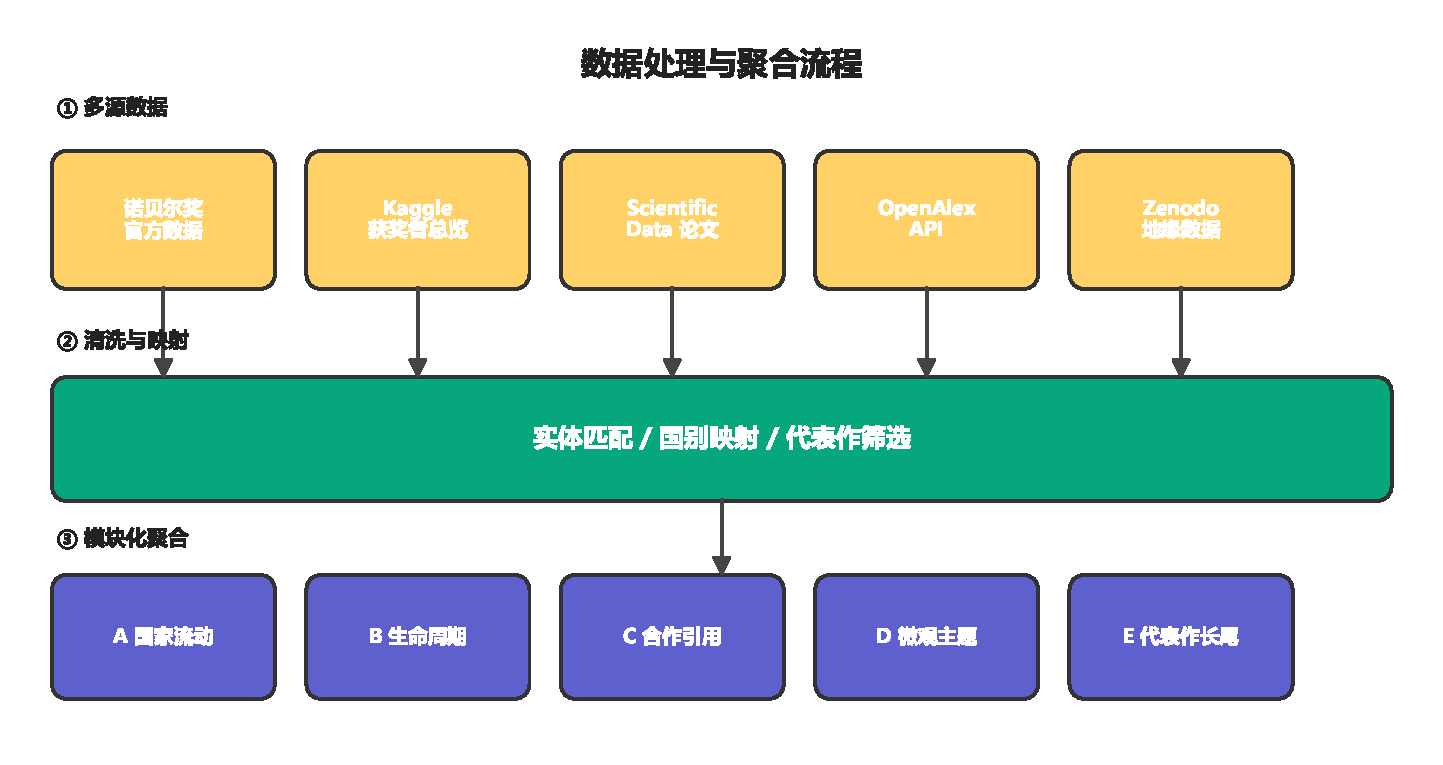
\includegraphics[width=0.85\linewidth]{pipeline.pdf}
    \caption{数据处理与聚合流程示意}
    \label{fig:pipeline}
\end{figure}

\section{可视化设计总览}
\subsection{设计理念}
本项目以"数据故事（Data Story）"为核心理念。我们首先将"如何拿诺奖"这一宽泛问题拆解为五个具体子问题，再为每个子问题设计最合适的可视化形式。

\subsection{模块架构}
项目由五个相互独立又彼此呼应的模块组成，分别对应五个研究问题。模块的命名、负责人与对应主题如\autoref{tab:modules}所示。
\begin{table}[H]
\centering
\caption{可视化模块分工表}
\label{tab:modules}
\begin{tabular}{clll}
\toprule
编号 & 负责人 & 可视化主题 & 回答的问题 \\
\midrule
A & 陈湘媛 & 地缘政治与空间轨迹 & 获奖者从哪里来，又流向哪些科学中心？\\
B & 黎子游 & 学术生命周期 & 代表作、产出高峰与获奖时间如何错位？\\
C & 谷帅志 & 合作网络与内部引用 & 得主之间的合作和引用如何连接知识共同体？\\
D & 张帅康 & 研究主题迁移与跨界 & 诺奖论文怎样跨越传统学科边界？\\
E & 游子力 & 代表作长尾影响力 & 代表作为什么能从普通论文中凸显出来？\\
F & 陈诣凡 & 参与报告写作 & —— \\
\bottomrule
\end{tabular}
\end{table}
\subsection{前端架构}
项目前端采用纯 HTML + CSS + JavaScript 技术栈，使用 D3.js v7 作为核心可视化库。整体页面采用"全屏逐页"叙事结构——用户通过滚轮、键盘方向键或点击右侧导航圆点在不同页面之间切换，每页承载一个完整的可视化模块。这种设计借鉴了 Tufte 对"数据—墨水比"和"叙事密度"的强调，通过减少装饰性元素、以数据本身驱动页面结构，使读者能够在短时间内获取完整的数据叙事。前端整体架构如\autoref{fig:architecture}所示。
\begin{figure}[H]
    \centering
    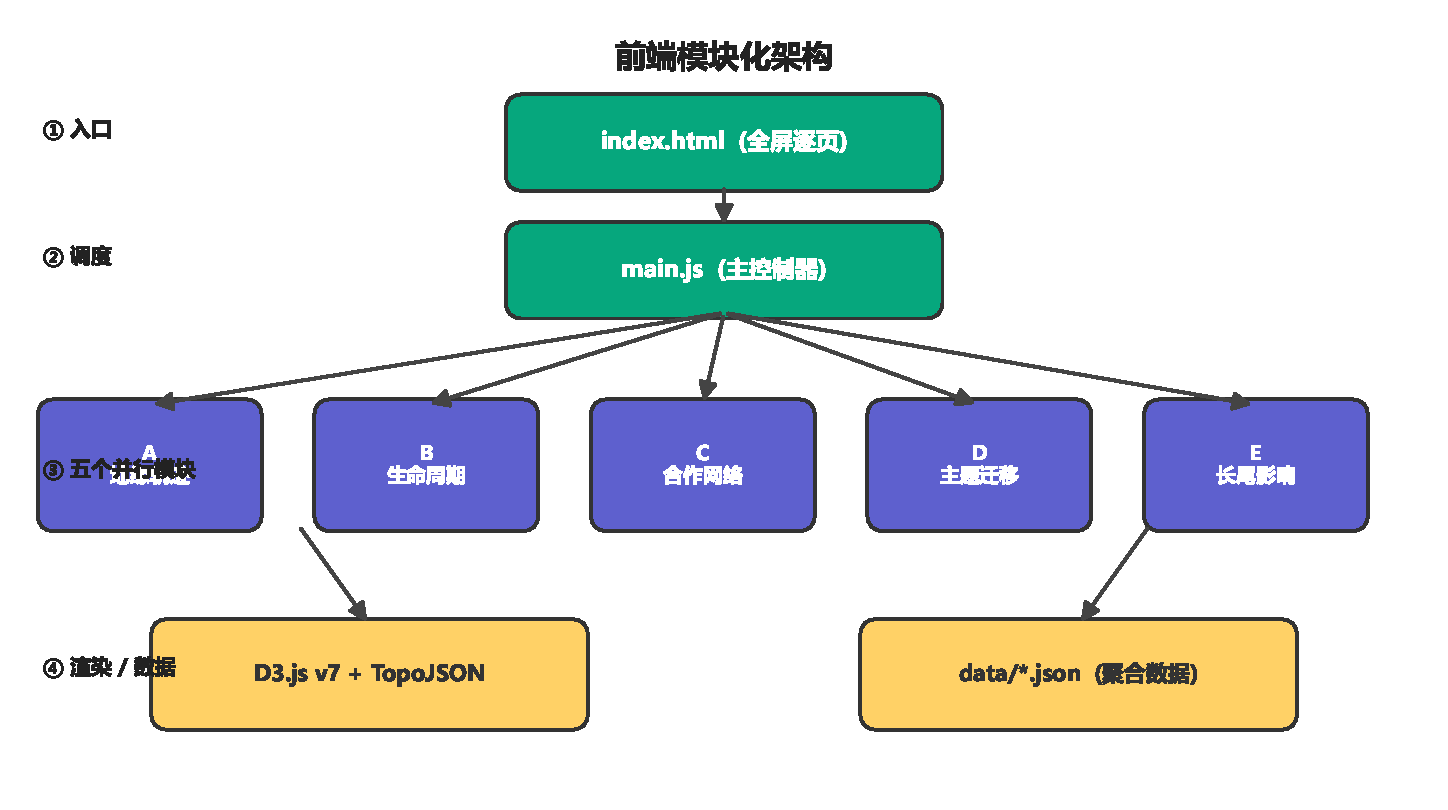
\includegraphics[width=0.85\linewidth]{architecture.pdf}
    \caption{前端模块化架构示意}
    \label{fig:architecture}
\end{figure}

\section{可视化模块实现}

\subsection{模块A：地缘政治与空间轨迹（负责人：陈湘媛）}

\subsubsection{设计目标}
模块A关注诺奖得主的"国籍流动"与"机构流动"，回答"获奖者从哪里来，又流向哪些科学中心"。本模块将诺奖得主置于宏观历史与空间结构中观察，不把获奖理解为单一的个人天赋结果，而是揭示出生地、学术机构所在国、历史阶段与国际流动如何共同构成"地图与时代的加成"。 可视化按"总览→空间流动→学术中心→历史身份→奖项演进"的递进逻辑组织，依次建立时间尺度、展示国家间人才迁移、解释成果产生地的变化、揭示国家身份背后的历史断层，并将学科变化放回地缘政治时期中比较。

\subsubsection{视图一：百年获奖节奏与学科版图（overview）}
该视图采用折线图与堆叠柱状图的组合形式，纵轴为获奖人数，横轴为年份（1901–2025）。数据处理时，将战争停发年份（如1940–1942年）的获奖人数显式标为零，使战争对奖项连续性的中断更加直观。\autoref{fig:moduleA_overview}展示了这一视图。

先沿顶部棕红色折线观察年度获奖总量的峰谷：总体趋势向上，但并非线性增加。两次世界大战期间（浅黄色竖带标记）奖项出现断档。下方堆叠柱按学科分类着色，清晰显示出物理学、化学、生理学或医学三大科学奖项长期构成主体；和平奖与文学奖穿插其中；经济学奖（1970年代后才纳入）则占据较窄的柱形。底部横向条形图汇总六大类别的百年总量，便于快速比较各学科的总体规模。交互上，鼠标悬停于趋势线可查看对应年份及各领域获奖详情，避免静态点位误导，也让年度结构信息更易读取。

\begin{figure}[H]
    \centering
    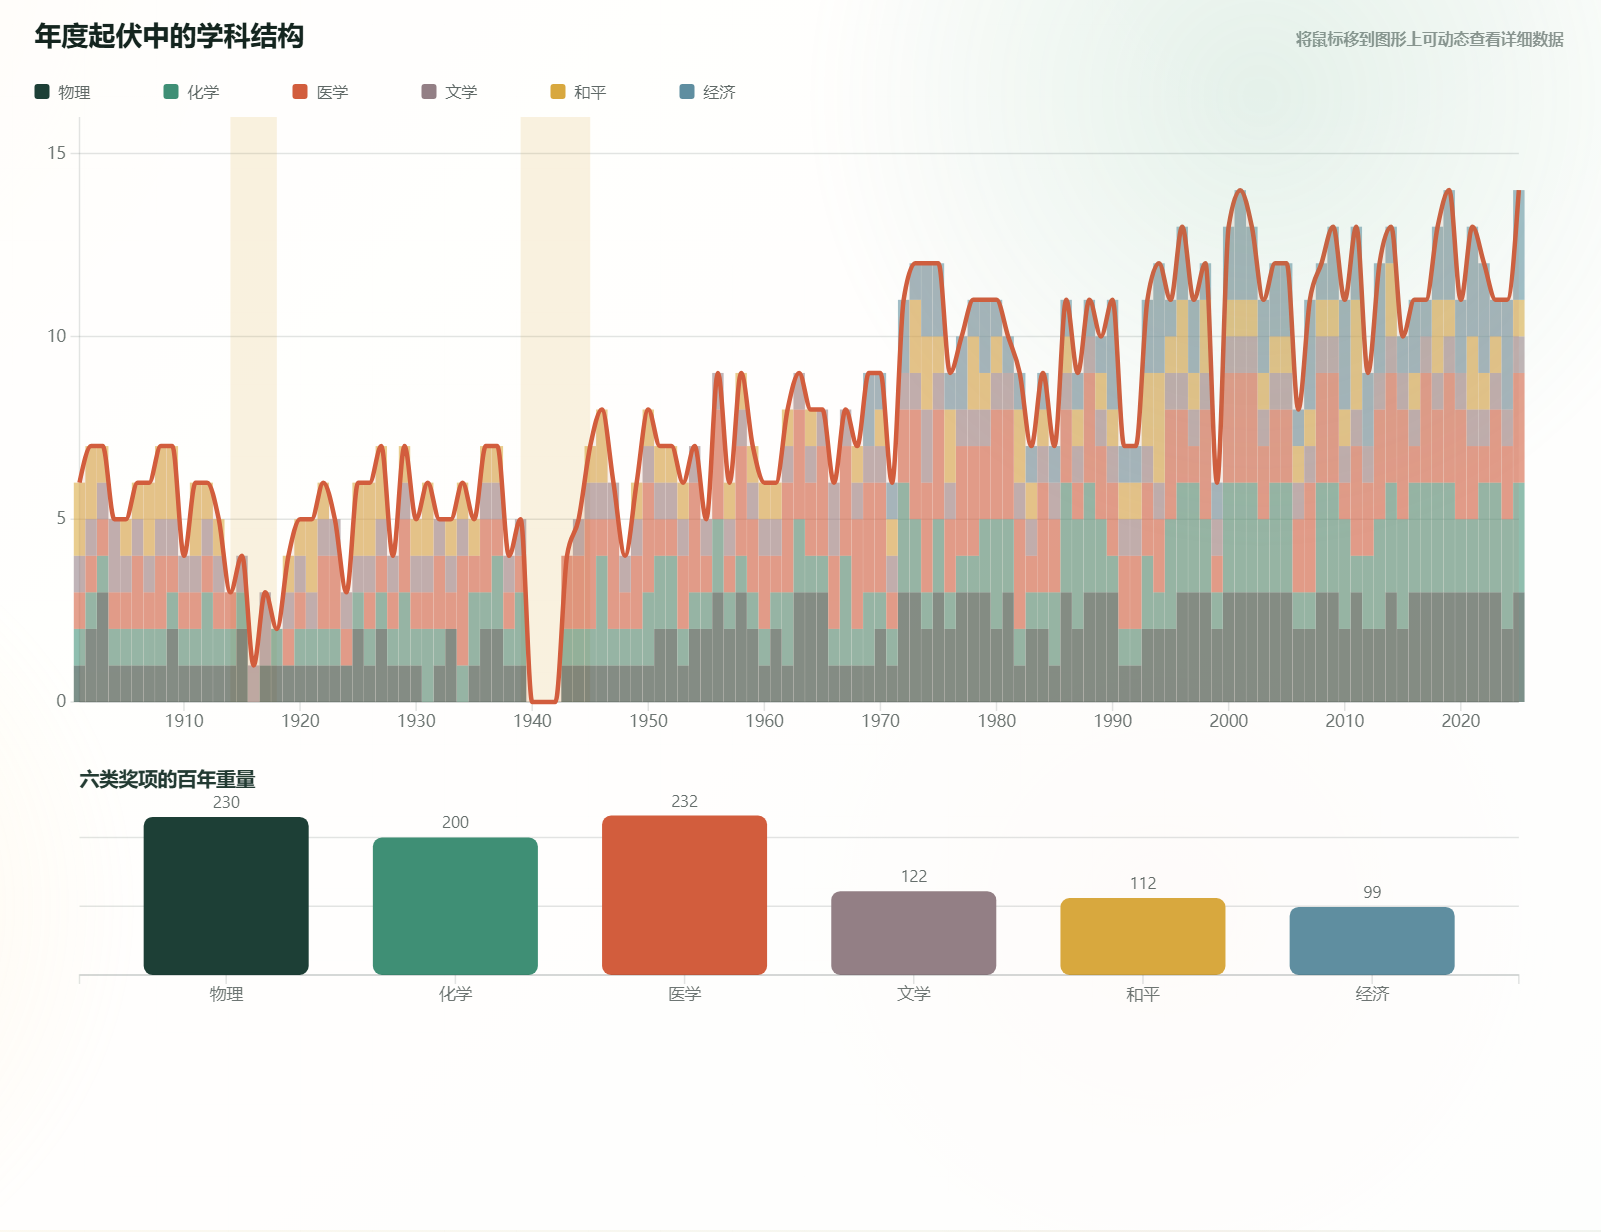
\includegraphics[width=\linewidth]{moduleA_overview.png}
    \caption{百年获奖节奏与学科版图（overview 视图）}
    \label{fig:moduleA_overview}
\end{figure}

\subsubsection{视图二：出生地→机构国的跨国迁移弧线（migration）}
该视图以世界地图为底图，用弧线（Arc）连接获奖者的出生国与获奖时所属机构国，线条越粗代表该路径上的流动人数越多。\autoref{fig:moduleA_migration}展示了这一视图。

弧线颜色编码流动类型：深绿色表示流向美国的迁移，红色表示跨洲流动，浅绿色表示其他跨国流动。用户可直观看出：欧洲内部的流动最为密集（欧洲大陆内弧线交织），而跨大西洋从欧洲流向美国的弧线最为粗壮。网页完整版中，该视图下方附带三层桑基路径图（Sankey），从左至右依次追踪"出生国→机构国→去世国"的完整人生轨迹，并辅以典型人生路径示例，帮助判断人才是否最终留在迁入地，也使抽象的流向转换为具体人物经历。 跨洲条形图则从宏观流向确认：欧洲到北美的迁移是最突出的跨洲流动。

\begin{figure}[H]
    \centering
    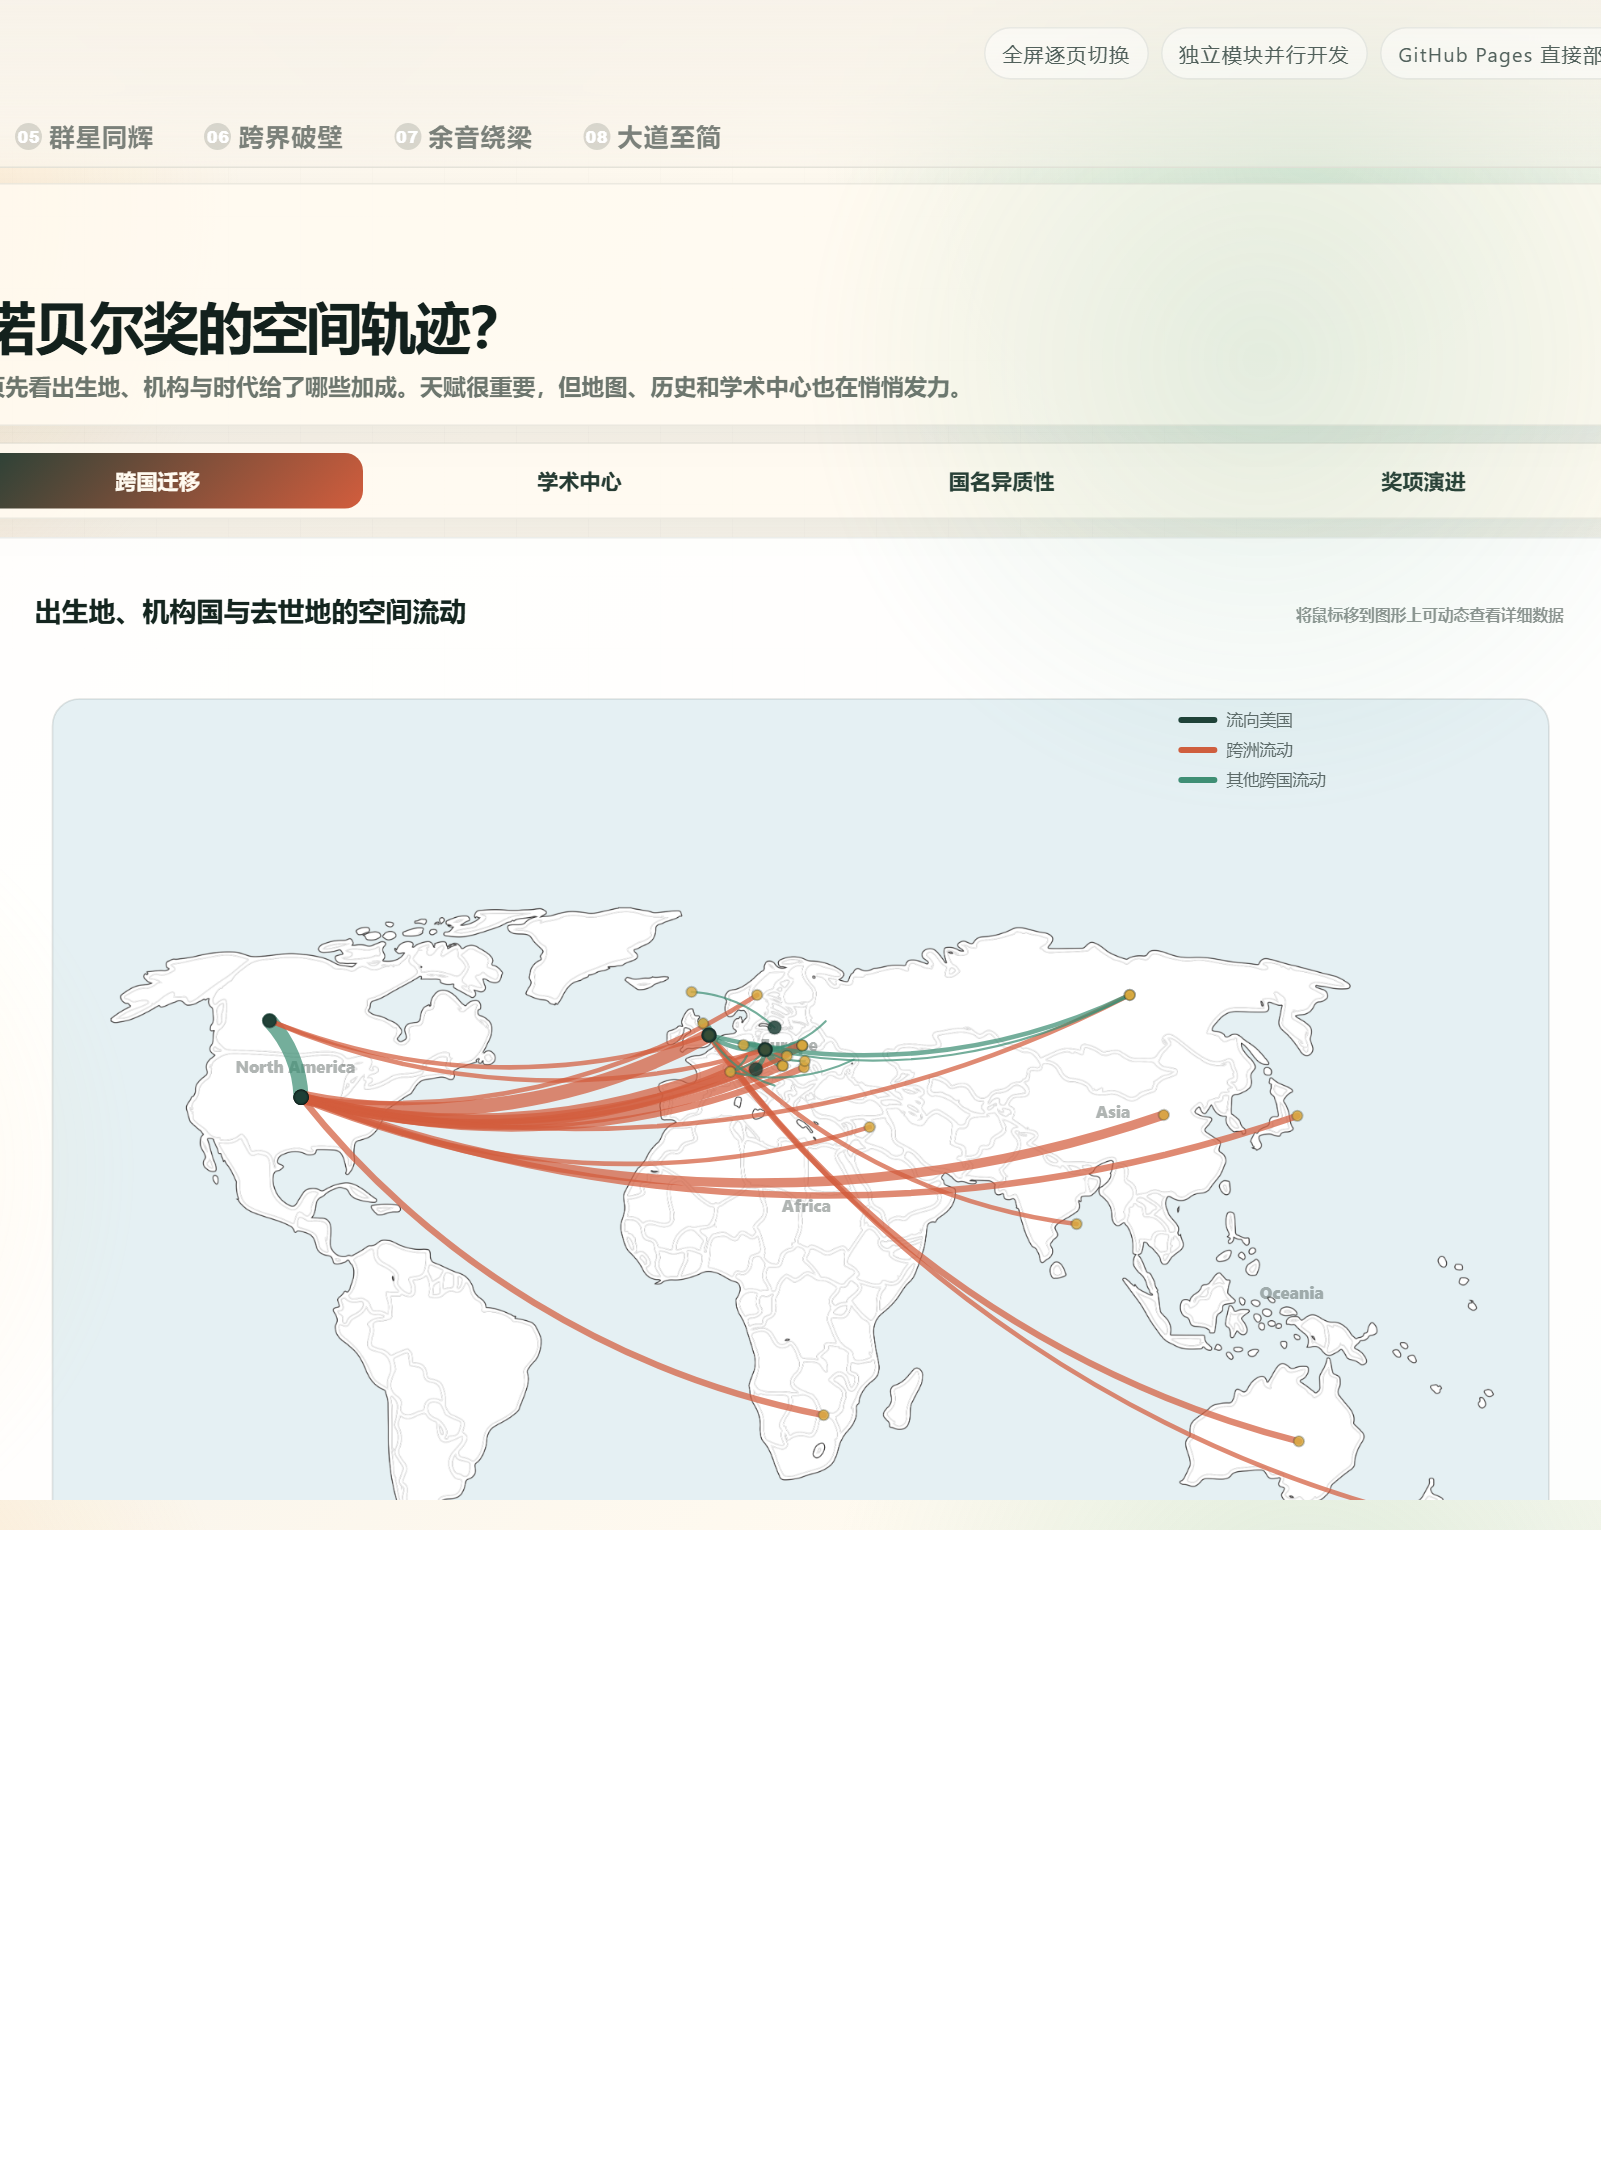
\includegraphics[width=\linewidth]{moduleA_migration.png}
    \caption{出生地→机构国的跨国迁移弧线（migration 视图）}
    \label{fig:moduleA_migration}
\end{figure}

\subsubsection{视图三：学术中心在历史时期的转移（centers）}
该视图按历史时期（1901–1913、1914–1918、1919–1938、1939–1945、1946–1962、1963–1979、1980–1991、1992–2025）分别统计各机构国吸纳的获奖者人数，以数字矩阵形式呈现，并通过分阶段比较与色块深浅强调学术中心的变化过程。图5展示了这一视图。\autoref{fig:moduleA_centers}展示了这一视图。

从矩阵可以清晰看到学术中心的位移轨迹：20世纪早期德国占据明显优势（1901–1913年德国12人、美国2人；1914–1918年德国3人、美国1人；1919–1938年德国17人、美国12人），英国紧随其后；二战后的1946–1962时期美国迅速上升至45人，此后持续领先，在1992–2025期间达到116人，保持压倒性优势。从"个人在哪里出生"推进到"成果在哪里产生"，这说明诺奖不仅奖励个人成就，也间接反映了世界科学资源在不同国家之间的重新分配。 网页完整版中，该视图下方附有气泡矩阵，纵轴列出出生洲、横轴列出机构国，气泡大小代表该洲向该机构国输送的获奖人数，直观反映了全球人才向美国（以及部分时期的英国、德国）汇集的格局。

\begin{figure}[H]
    \centering
    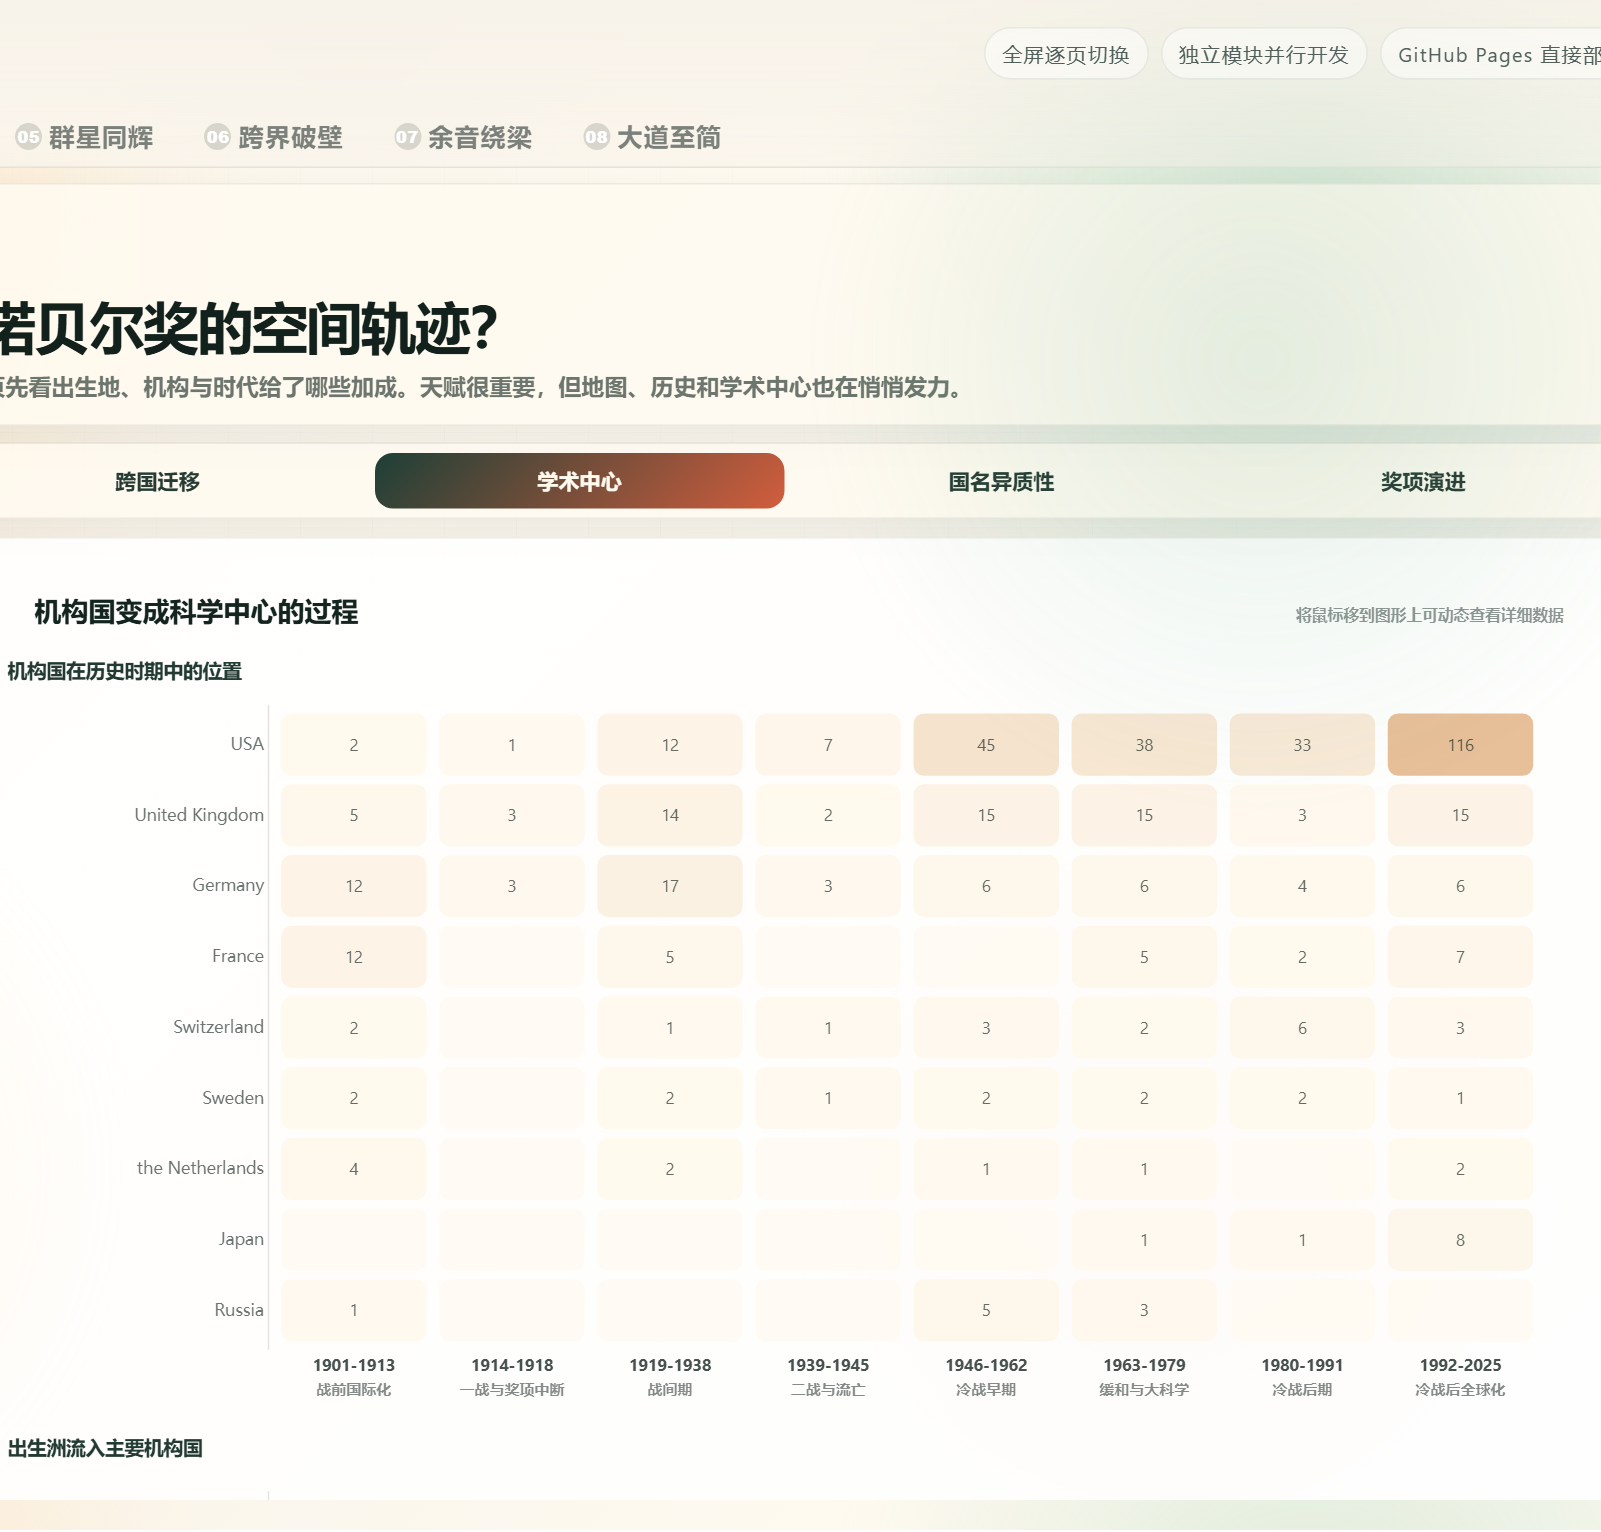
\includegraphics[width=\linewidth]{moduleA_centers.png}
    \caption{学术中心在历史时期的转移（centers 视图）}
    \label{fig:moduleA_centers}
\end{figure}

\subsubsection{视图四：历史国名与现代国家的映射（identity）}
部分获奖者出生时的国家已在历史中消失或重组（如奥匈帝国、普鲁士、苏联、英属印度等）。该视图使用线性流图（Linear Flow Diagram）展示历史政体与现代国家之间的映射关系。\autoref{fig:moduleA_identity}展示了这一视图。

左侧节点为历史政体名称（如"大英帝国/联合王国版图""德意志帝国""俄罗斯帝国""苏联""奥匈帝国"等），右侧节点为对应的现代国家。节点之间的连线越粗，说明该历史政体下出生的获奖者在现代国家中被识别的数量越多。底部排行榜列出了映射人数最多的历史政体——大英帝国和苏联位居前列，反映了帝国解体、殖民地独立、国家边界重组与冷战格局对诺奖得主地域身份的深层影响。

\begin{figure}[H]
    \centering
    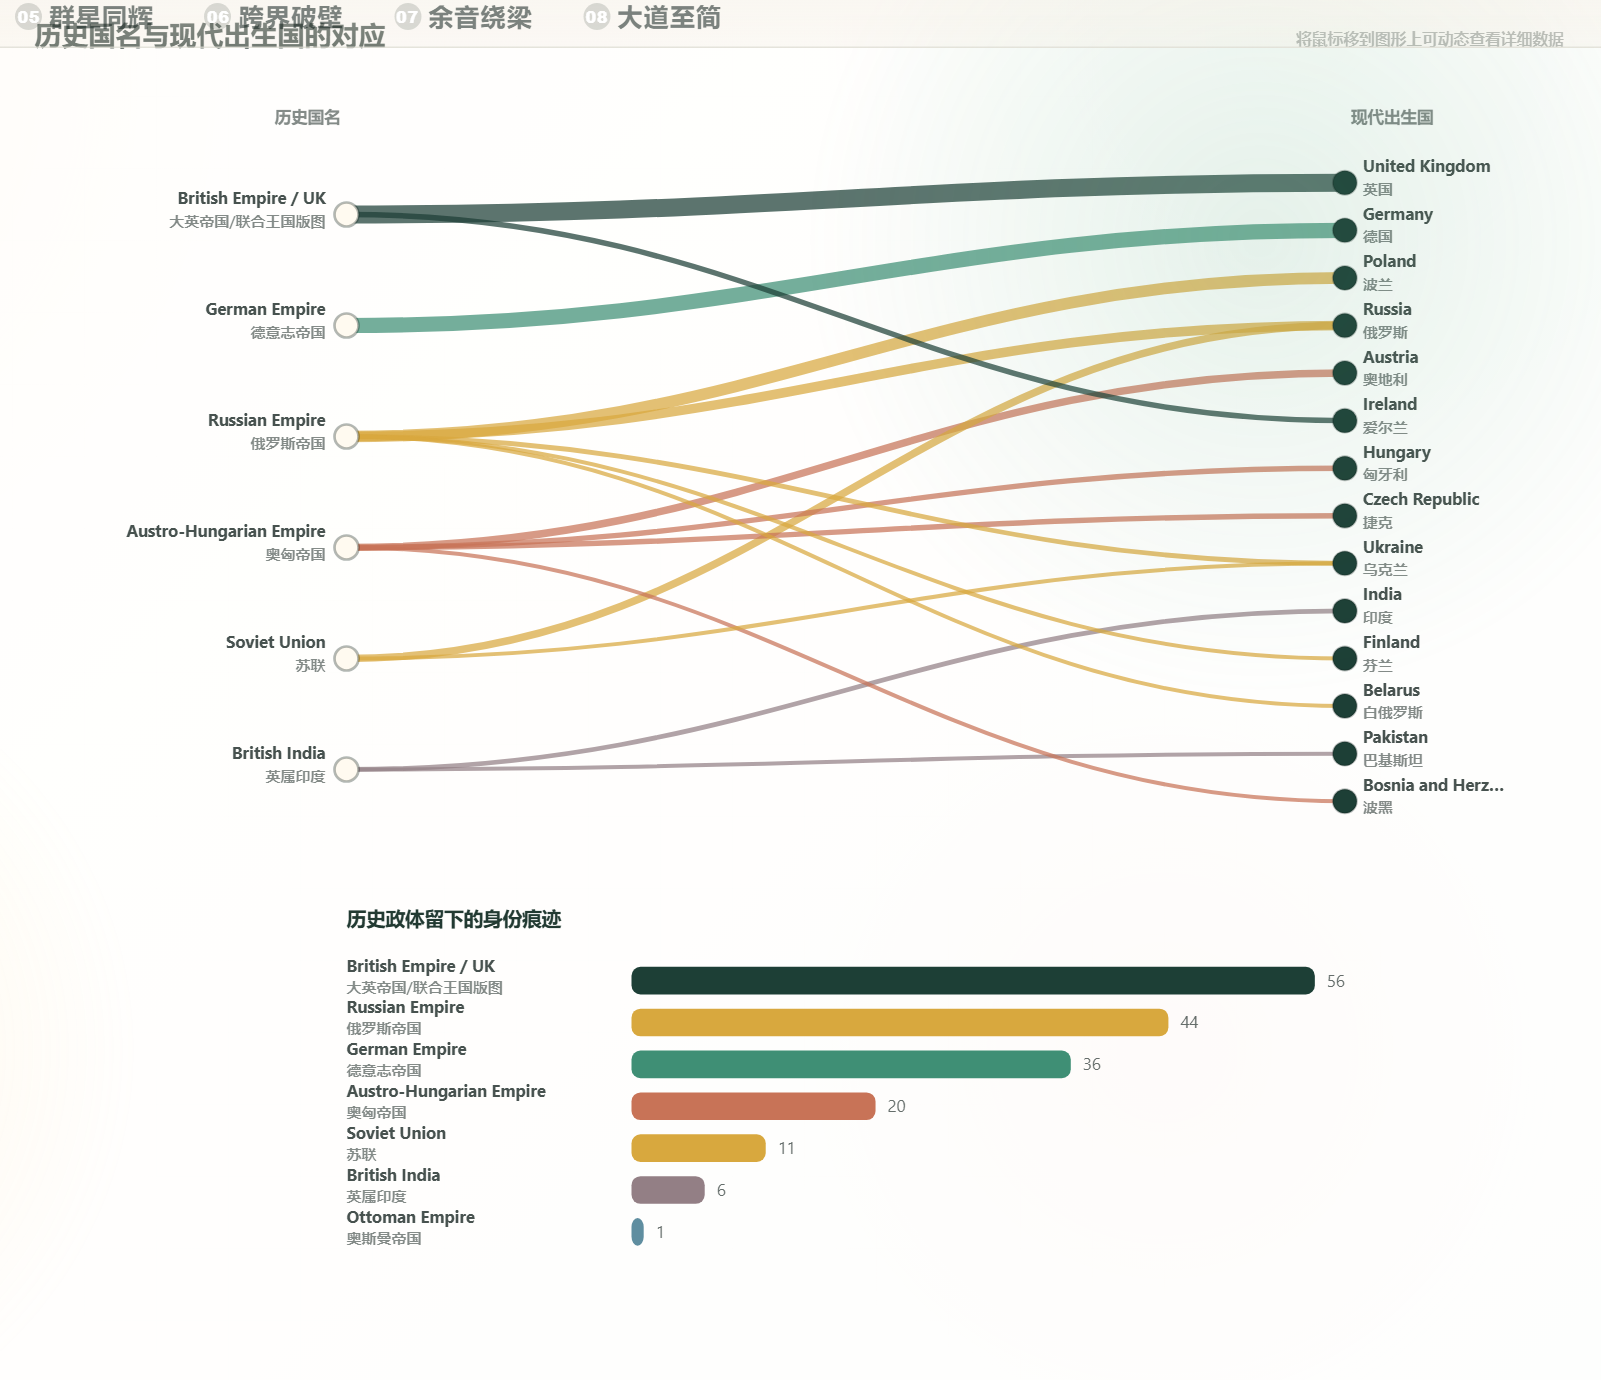
\includegraphics[width=\linewidth]{moduleA_identity.png}
    \caption{历史国名与现代国家的映射（identity 视图）}
    \label{fig:moduleA_identity}
\end{figure}

\subsubsection{视图五：奖项河流中的时代断点（periods）}
该视图采用河流图（Streamgraph）结合阶段性分类，将奖项演进历程划分为"世界大战""冷战早期""冷战后期""全球化调整"等历史阶段。\autoref{fig:moduleA_periods}展示了这一视图。

每条彩色"河流"代表一个奖项类别，河流宽度对应该类获奖记录在该时期的数量占比。世界大战阶段的河流明显收窄甚至中断；冷战早期以物理学和化学为主导；冷战后期医学类奖项的河流逐渐加宽；全球化时期经济学奖的贡献占比明显上升，和平奖与文学奖的占比则相对收窄。交互上，鼠标悬停于某一领域时仅高亮显示该领域在当前年份的比例，而非一次性展示所有领域，从而降低信息噪音，使读者更易追踪单一学科的长期趋势。 视图底部的时间线单独标出停发年份（如1915–1919、1940–1942等），用于解释河流图中的断裂与变窄现象。

\begin{figure}[H]
    \centering
    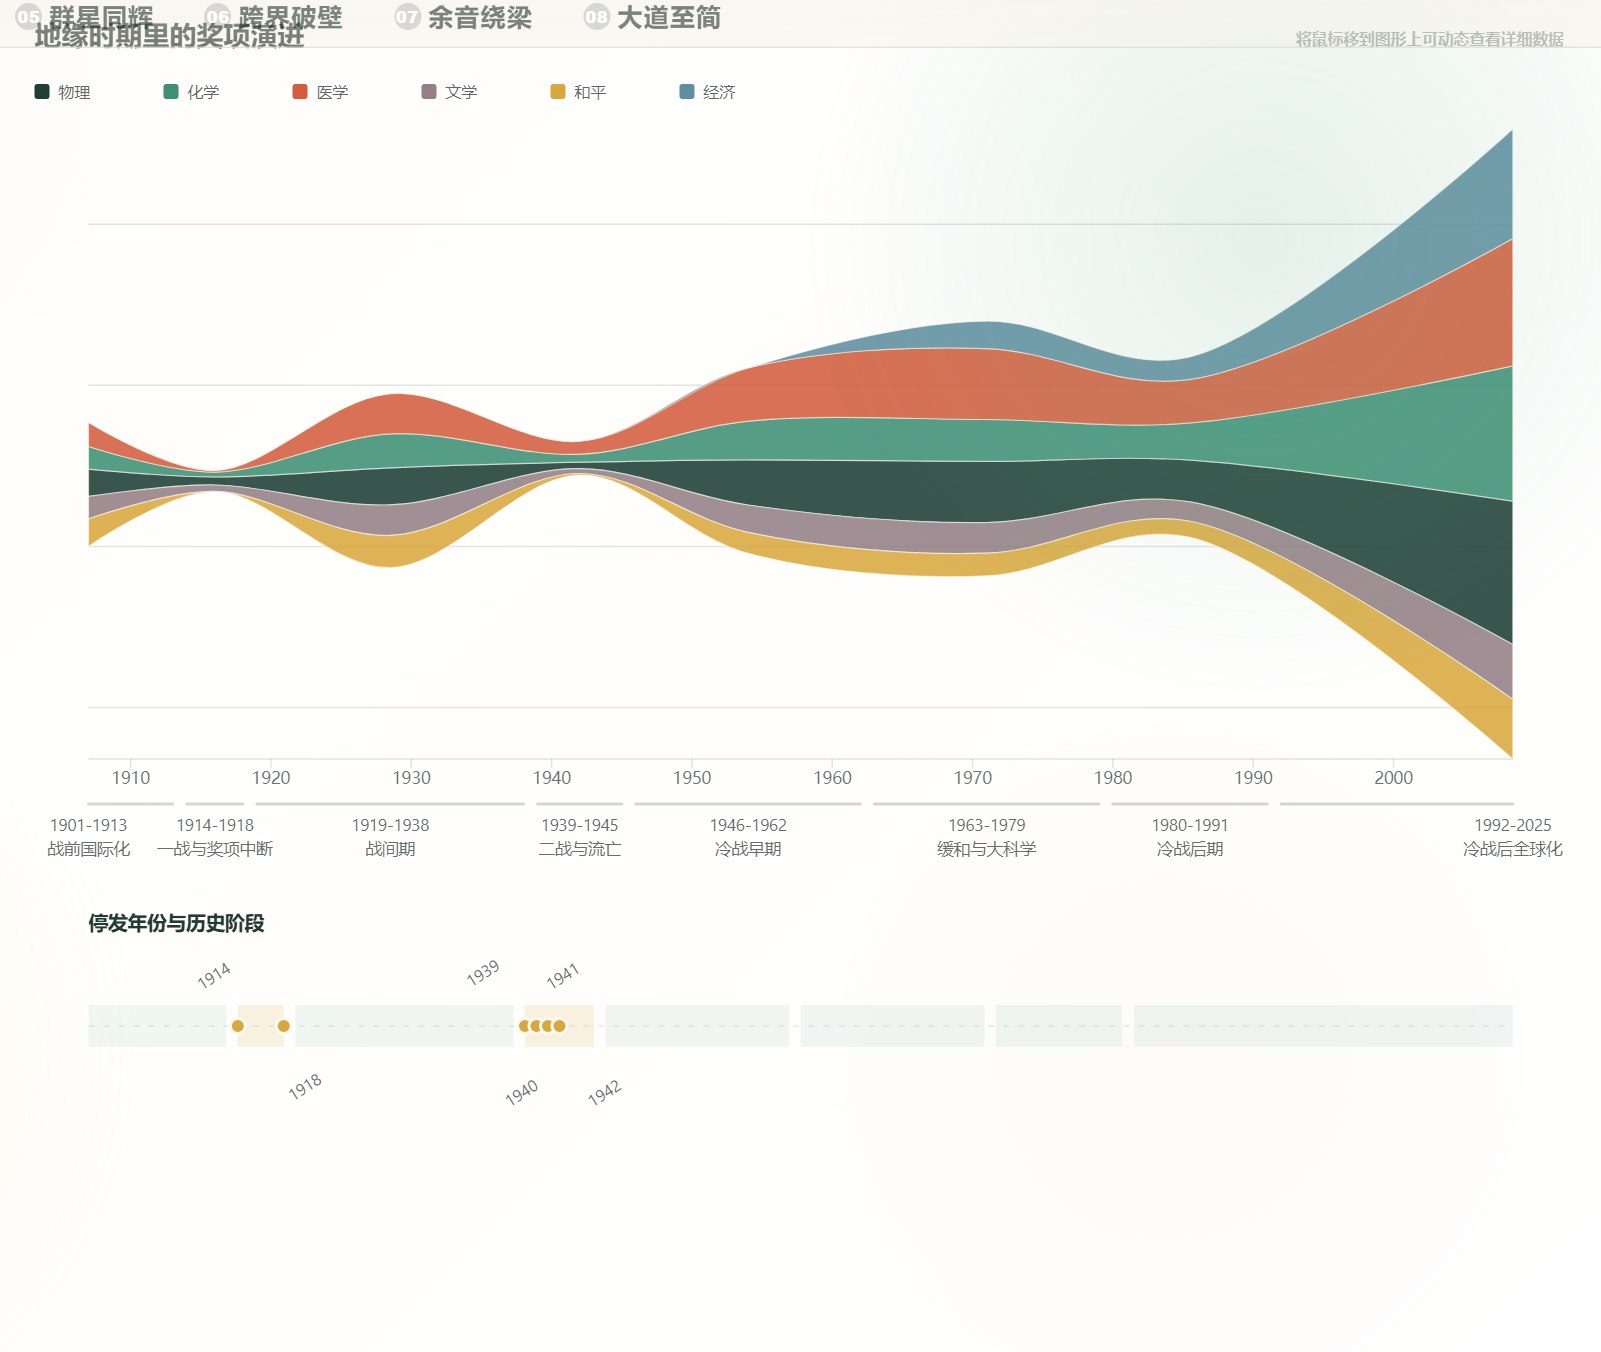
\includegraphics[width=\linewidth]{moduleA_periods.png}
    \caption{奖项河流中的时代断点（periods 视图）}
    \label{fig:moduleA_periods}
\end{figure}

\subsubsection{主要发现}
通过模块 A 的可视化，我们观察到以下三个主要现象：
\begin{enumerate}
    \item \textbf{科学中心高度集中且发生转移}：20世纪早期科学中心呈现欧洲主导格局，德国在1901–1938年间显著领先于美国；二战后美国迅速成为绝对主导的学术中心，吸纳了全球最多的跨国科学家。
    \item \textbf{20 世纪中叶的"美国化"浪潮}：跨大西洋弧线最粗的方向是从英、法、德等欧洲国家流向美国。大量欧洲科学家在二战后迁入美国，使美国成为 1945 年后最大的"诺奖进口国"。这种人才虹吸与二战期间欧洲科研体系遭遇破坏、美国加大科研投入密切相关。
    \item \textbf{亚洲崛起与科学多极化趋势}：21世纪以来，日本在诺奖得主数量上显著上升（1992–2025年达8人）。尽管亚洲整体绝对数量仍远少于欧美，但增长趋势明显，反映了全球科学多极化的新时代特征。中国（大陆与港澳台地区）与韩国等也在近年实现突破，该趋势在网页完整版的地缘数据中有进一步体现。历史国名映射视图也揭示：帝国解体后，原属大英帝国和苏联地区的得主在现代国家中分布广泛，其人才红利被多个新生国家共享。
    \item \textbf{地图与时代的加成}：综合以上视图可见，诺奖并非仅由个人天赋决定。获奖者的空间轨迹深刻受到出生地、教育与研究机构所在国的科研资源、历史阶段（战争、冷战、帝国解体）和国际流动机会的共同影响。"如何拿诺奖"首先需要杰出的研究能力，但进入高密度科学中心、抓住特定历史窗口，同样是不可忽视的结构性加成。
\end{enumerate}

\subsection{模块B：学术生命周期（负责人：黎子游）}

\subsubsection{设计目标}
模块B 以学术生涯相对时间为横轴，将每位诺奖得主的论文产出轨迹、代表作发表时间与获奖事件叠加在同一条时间线上，回答"代表作、产出高峰与获奖时间如何错位"。模块共包含七个交互视图，通过D3.js 的面积图、堆叠柱状图、折线图、散点图与雷达图等多种图表类型呈现。

\subsubsection{视图一：学术轨迹对齐（trajectory）}
该视图将物理、化学、医学三个学科的获奖者以首篇论文发表时间为原点（T+0）进行对齐，纵轴为平均年发表量，横轴为学术生涯相对时间（T+0至T+60年）。\autoref{fig:moduleB_trajectory}展示了这一视图。

曲线在某个时间段的隆起代表该时期的论文产出高峰。视图中用标记线标示了平均获奖时间（T+28）与黄金创作期（T+28），产出高峰主要集中在T+20至T+35之间。平均学术生涯长度约为48年。下方折线图同步展示引用影响力趋势，可见FWCI在生涯早期（T+5左右）出现峰值，随后逐步回落。

\begin{figure}[H]
    \centering
    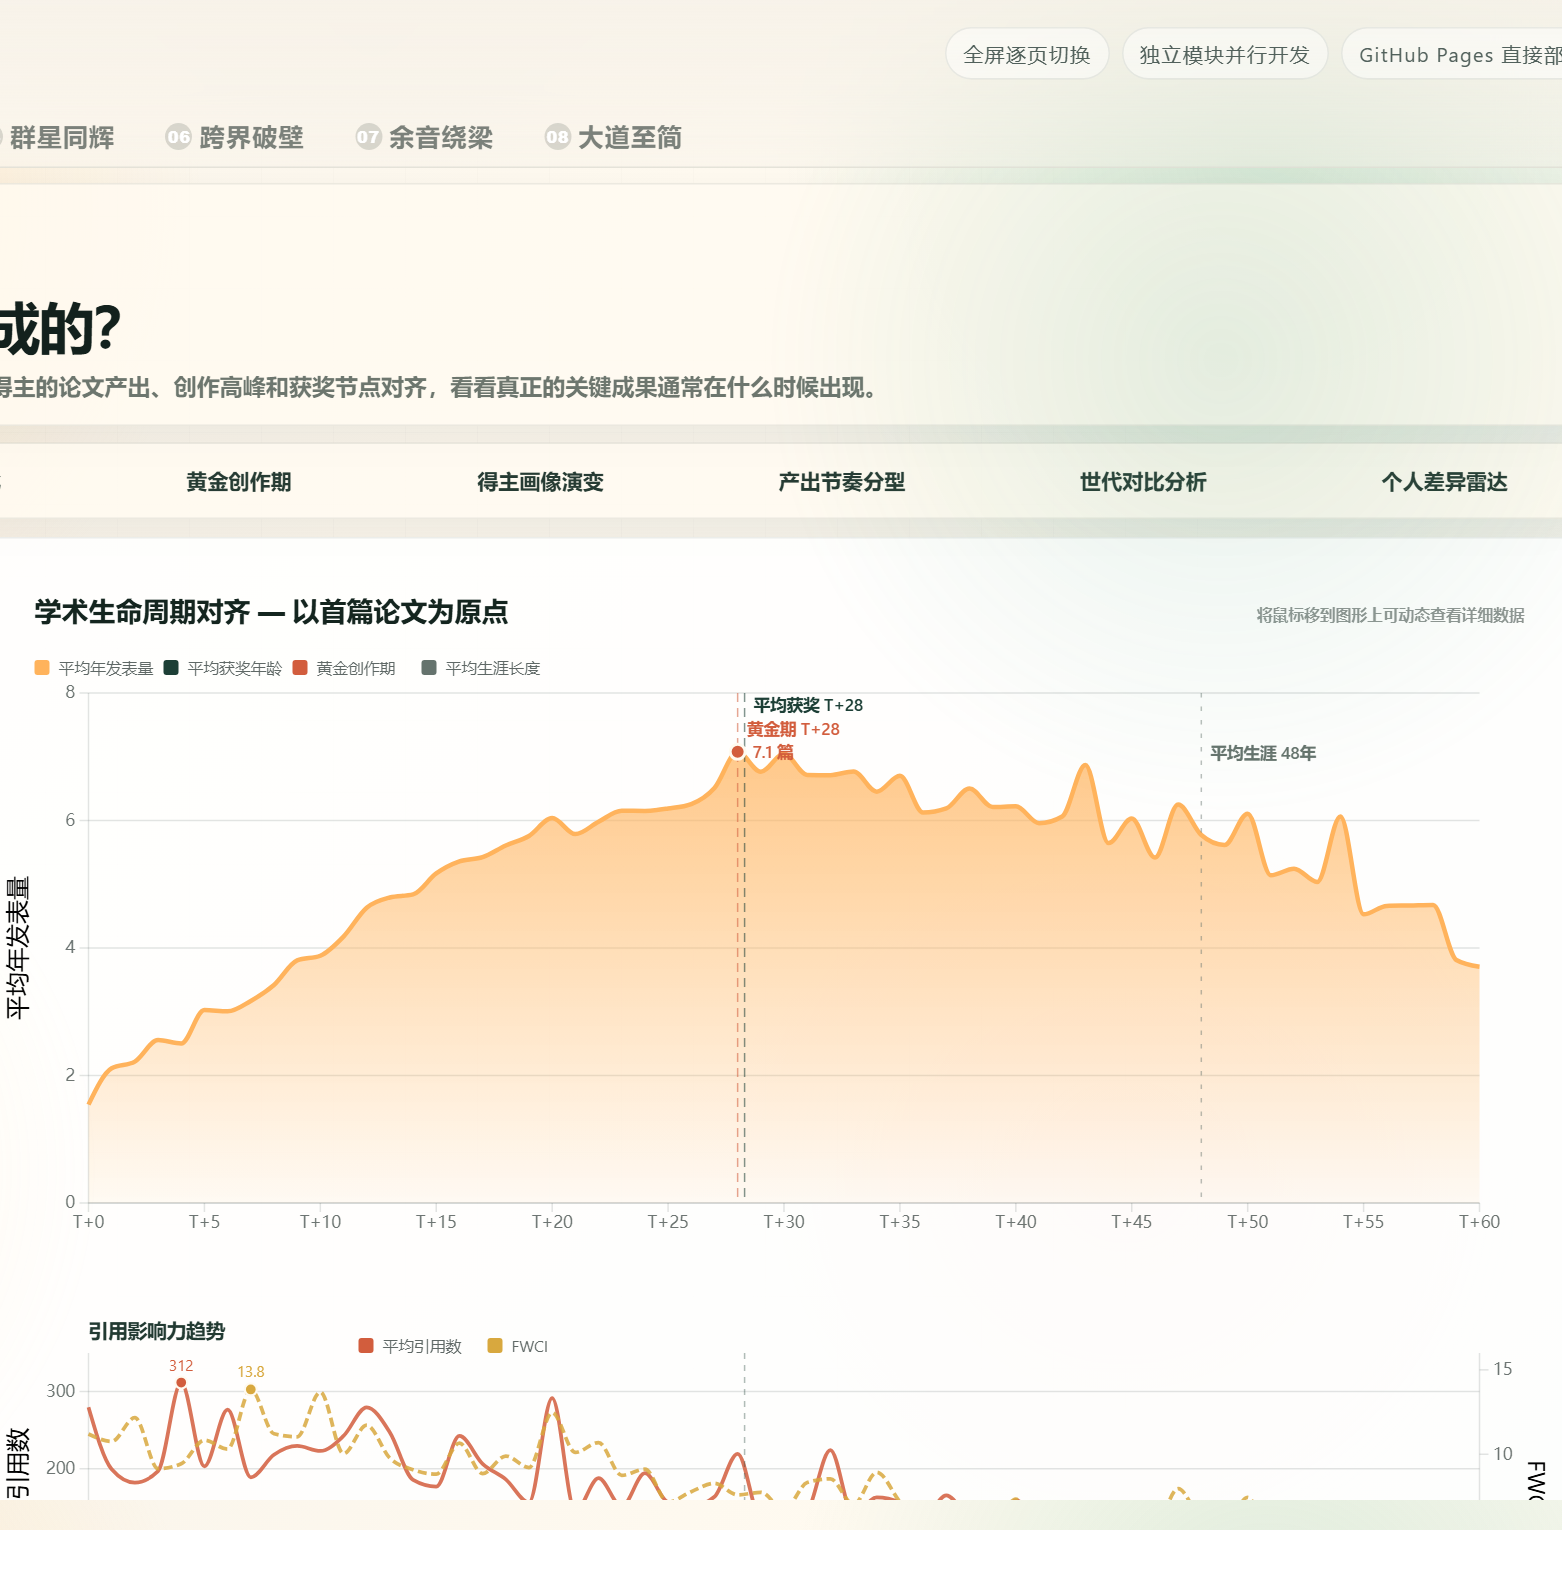
\includegraphics[width=\linewidth]{moduleB_trajectory.png}
    \caption{学术轨迹对齐：论文产出年龄分布与获奖节点（trajectory 视图）}
    \label{fig:moduleB_trajectory}
\end{figure}

\subsubsection{视图二：获奖前后对比（comparison）}
该视图以获奖年份为分界点，将所有得主的论文产出划分为"获奖前"与"获奖后"两个阶段，用堆叠柱状图展示平均产出量变化。\autoref{fig:moduleB_comparison}展示了这一视图。

观察发现，三大科学类别的得主在获奖前的平均论文产出均显著高于获奖后（物理学：获奖前65篇 vs 获奖后47篇；化学：获奖前160篇 vs 获奖后101篇；医学：获奖前88篇 vs 获奖后67篇）。物理学和化学的获奖后产出下降尤为明显，而医学类得主的下降幅度相对较小。这表明诺贝尔奖更多是在"确认已经产生的影响力"而非"开启新的研究高峰"——获奖后得主可能面临更多的社会事务、行政职责和公众关注，从而减少了直接从事前沿研究的时间。

\begin{figure}[H]
    \centering
    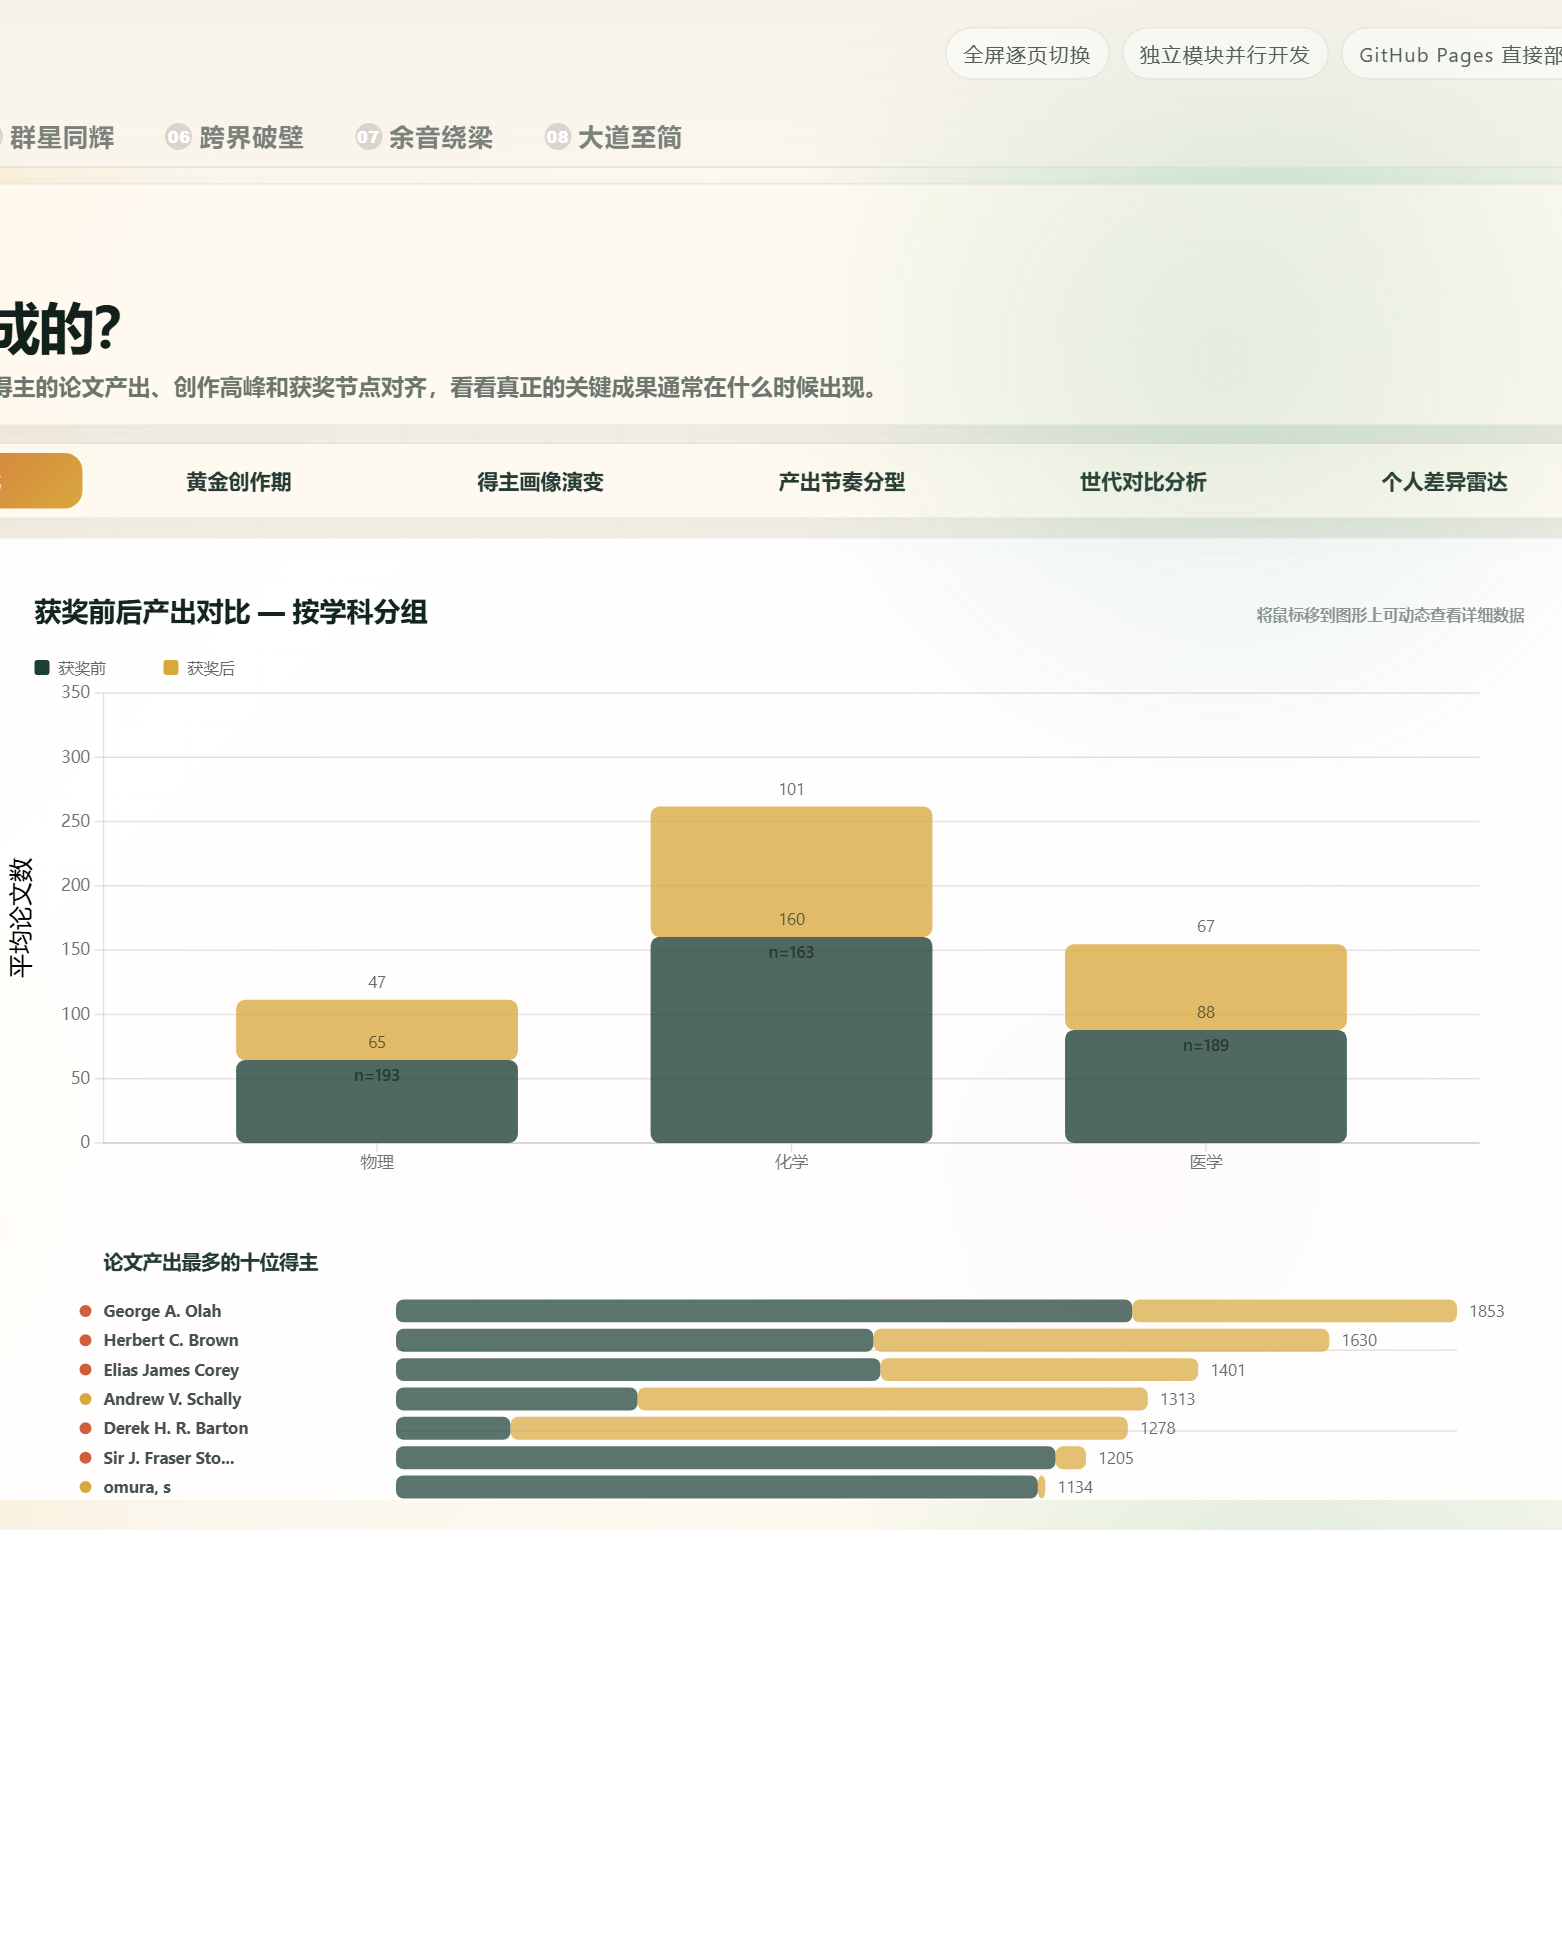
\includegraphics[width=\linewidth]{moduleB_comparison.png}
    \caption{获奖前后论文产出对比（comparison 视图）}
    \label{fig:moduleB_comparison}
\end{figure}

\subsubsection{视图三：黄金创作期热力图（heatmap）}
该视图以年份与年代为横轴、高峰期得主人数为纵轴，通过折线图与柱状图组合展示不同时期论文产出高峰的分布特征。\autoref{fig:moduleB_heatmap}展示了这一视图。

上方折线图显示各年份处于产出高峰期的得主人数波动，2010年达到峰值（20人）；下方柱状图汇总各年代高峰得主人数，1990年代（108人）与1980年代（103人）为高峰期最集中的年代。最下方的学科分组图显示，化学与医学的高峰期分布较物理更为分散。这反映了科学共同体规模的扩大，以及现代科研体系对科学家产出周期的延长效应。

\begin{figure}[H]
    \centering
    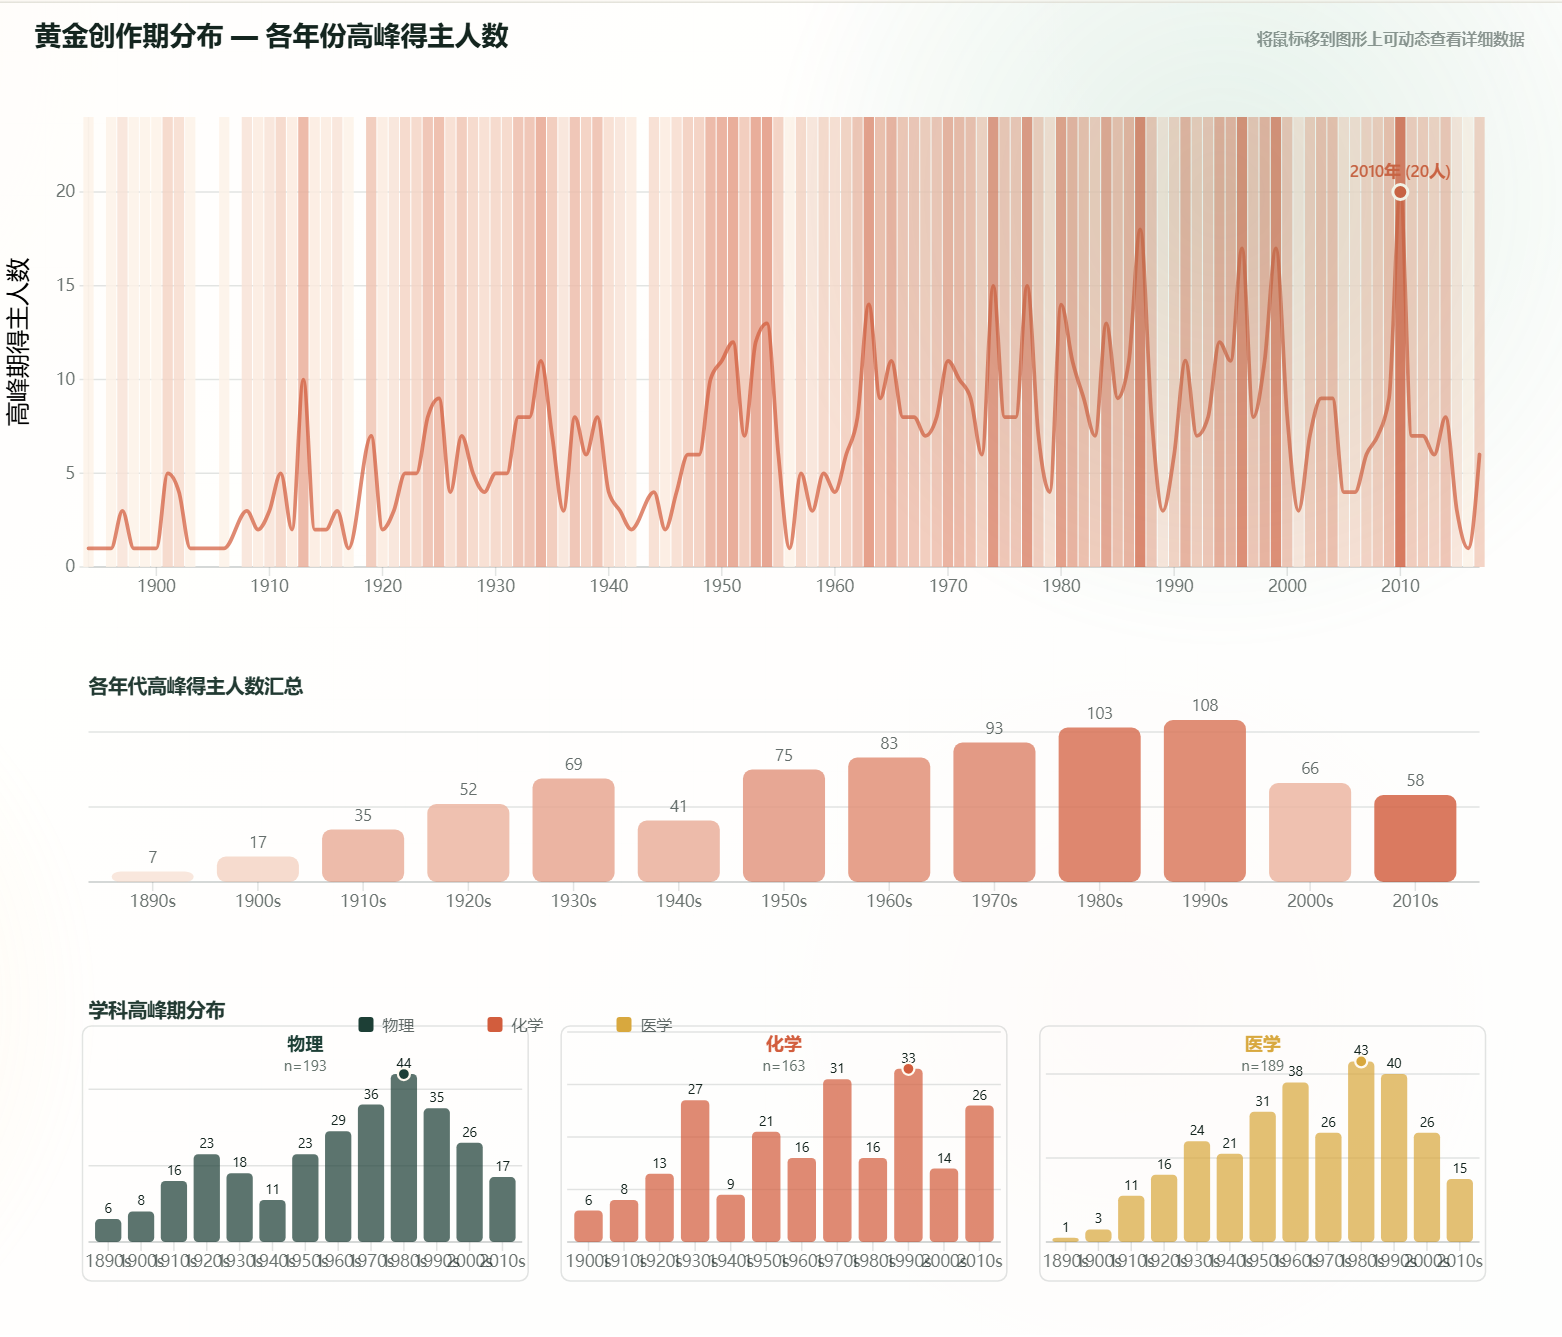
\includegraphics[width=\linewidth]{moduleB_heatmap.png}
    \caption{黄金创作期热力图（heatmap 视图）}
    \label{fig:moduleB_heatmap}
\end{figure}

\subsubsection{视图四：得主画像随年代演化（evolution）}
该视图使用曲线图，按获奖年代展示不同时期得主的平均特征：获奖年龄、论文总数、代表作被引次数等。\autoref{fig:moduleB_evolution}展示了这一视图。

随着年代推移，三项关键指标均呈上升趋势：1900--1920 年代得主平均获奖年龄约 50 岁，2020 年代已推迟至 65 岁以上；论文总数从早期的每人 20~30 篇增长至近期的 100~200 篇；代表作被引次数也呈指数级增长。这些变化说明诺贝尔奖越来越依赖"长期积累"，个人天才叙事正在被制度化、团队化的科研体系所改写。

\begin{figure}[H]
    \centering
    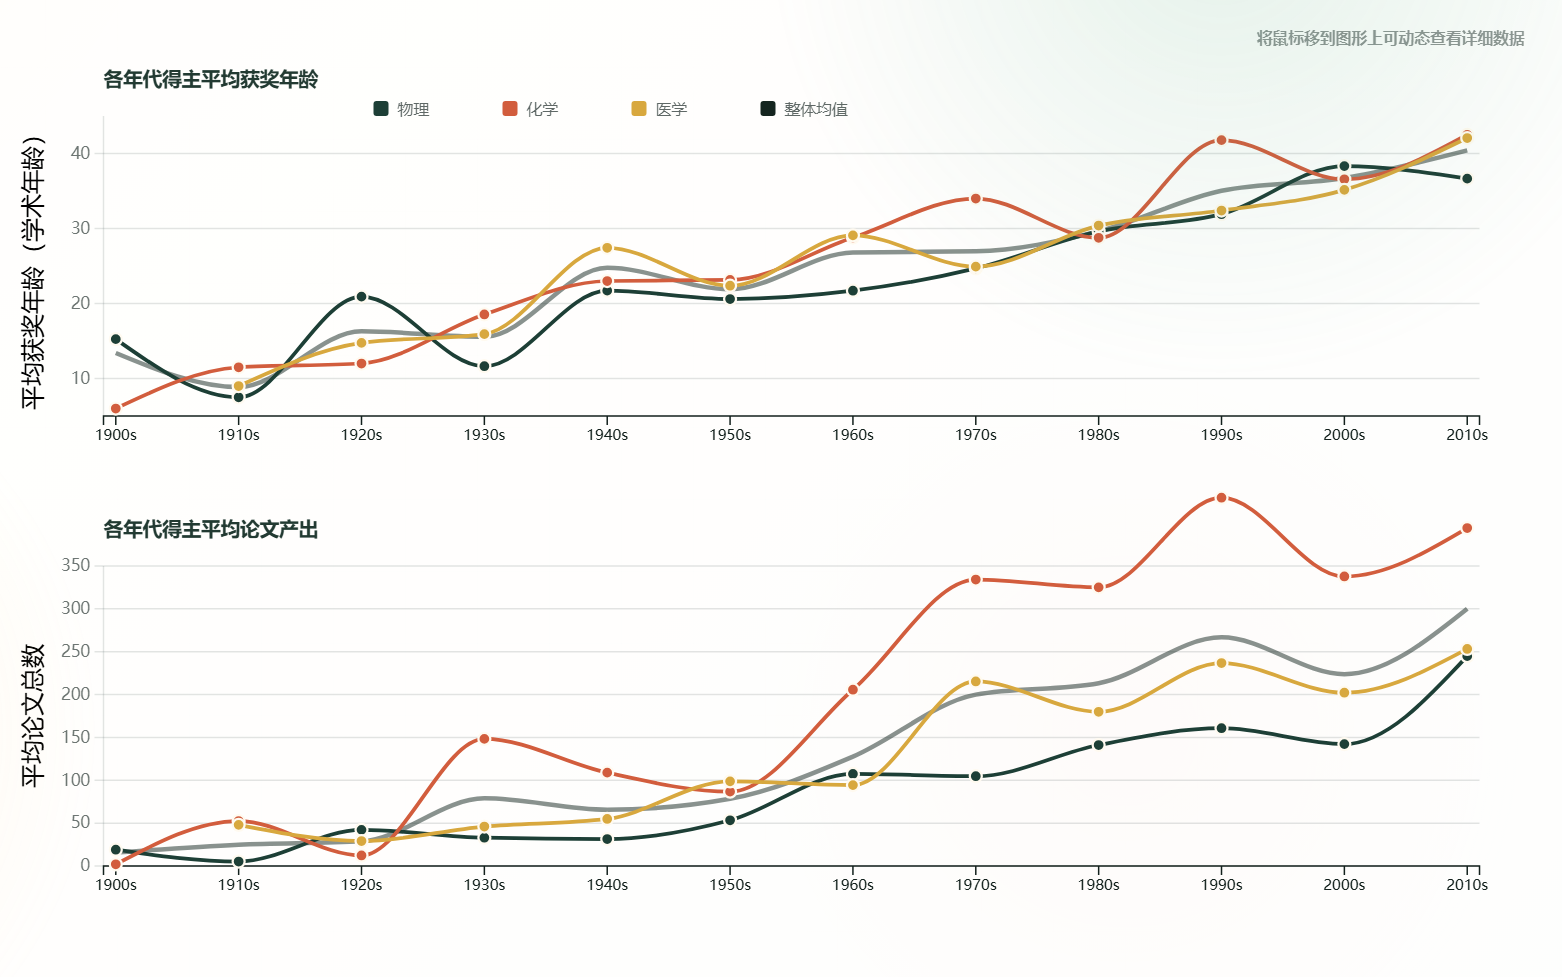
\includegraphics[width=\linewidth]{moduleB_evolution.png}
    \caption{得主画像随年代演化（evolution 视图）}
    \label{fig:moduleB_evolution}
\end{figure}

\subsubsection{视图五：个体产出节奏分型（rhythm）}
该视图通过产出集中度散点图与典型节奏示例面积图展示每位得主的论文产出分布特征。\autoref{fig:moduleB_rhythm}展示了这一视图。

上方散点图显示各学科得主前3年产出占总产出的比例（物理均值0.27，化学0.19，医学0.17），反映产出集中度的学科差异；下方6个示例呈现不同的个体产出节奏——有的呈现尖锐单峰（如Fitch，集中度0.36），有的分布平缓（如Townes，集中度0.04）。物理学中高集中度的"单峰爆发"模式更为常见，而医学类得主更多呈现低集中度的平缓分布，反映了不同学科的科研范式差异：物理学的重大发现常由年轻科学家在短期内完成，而医学和生物学突破往往需要长时间的实验积累。

\begin{figure}[H]
    \centering
    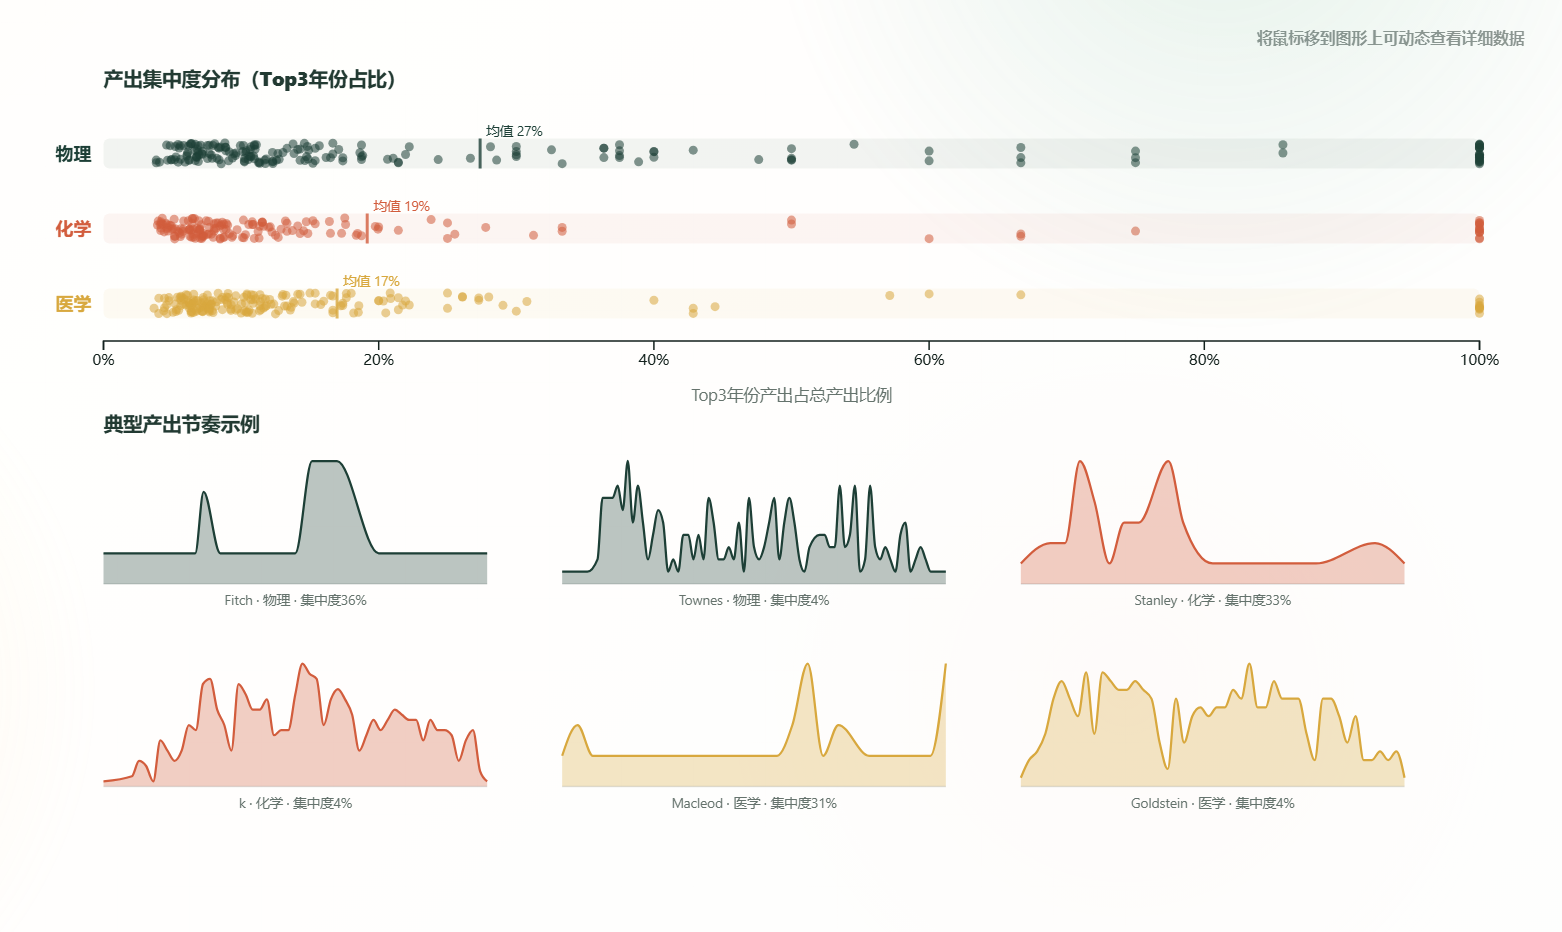
\includegraphics[width=\linewidth]{moduleB_rhythm.png}
    \caption{个体产出节奏分型：突破型与积累型（rhythm 视图）}
    \label{fig:moduleB_rhythm}
\end{figure}

\subsubsection{视图六：出生世代比较（cohort）}
该视图按得主的出生年代分组（1880s、1890s、…、1970s），以色块矩阵比较不同世代的平均获奖年龄（学术年龄，即首篇论文发表至获奖的间隔年数）与平均学术生涯长度。\autoref{fig:moduleB_cohort}展示了这一视图。

矩阵清楚显示：越晚出生的世代，从首篇论文发表到获奖的间隔越长（物理学科从1880s的16年延长至1930s的34年；化学从1860s的19年延长至1940s的37年）。这种趋势与科研训练周期延长、学科深度增加以及诺奖评选的滞后性有关——现代诺奖越来越倾向于"验证影响而非发现本身"。

\begin{figure}[H]
    \centering
    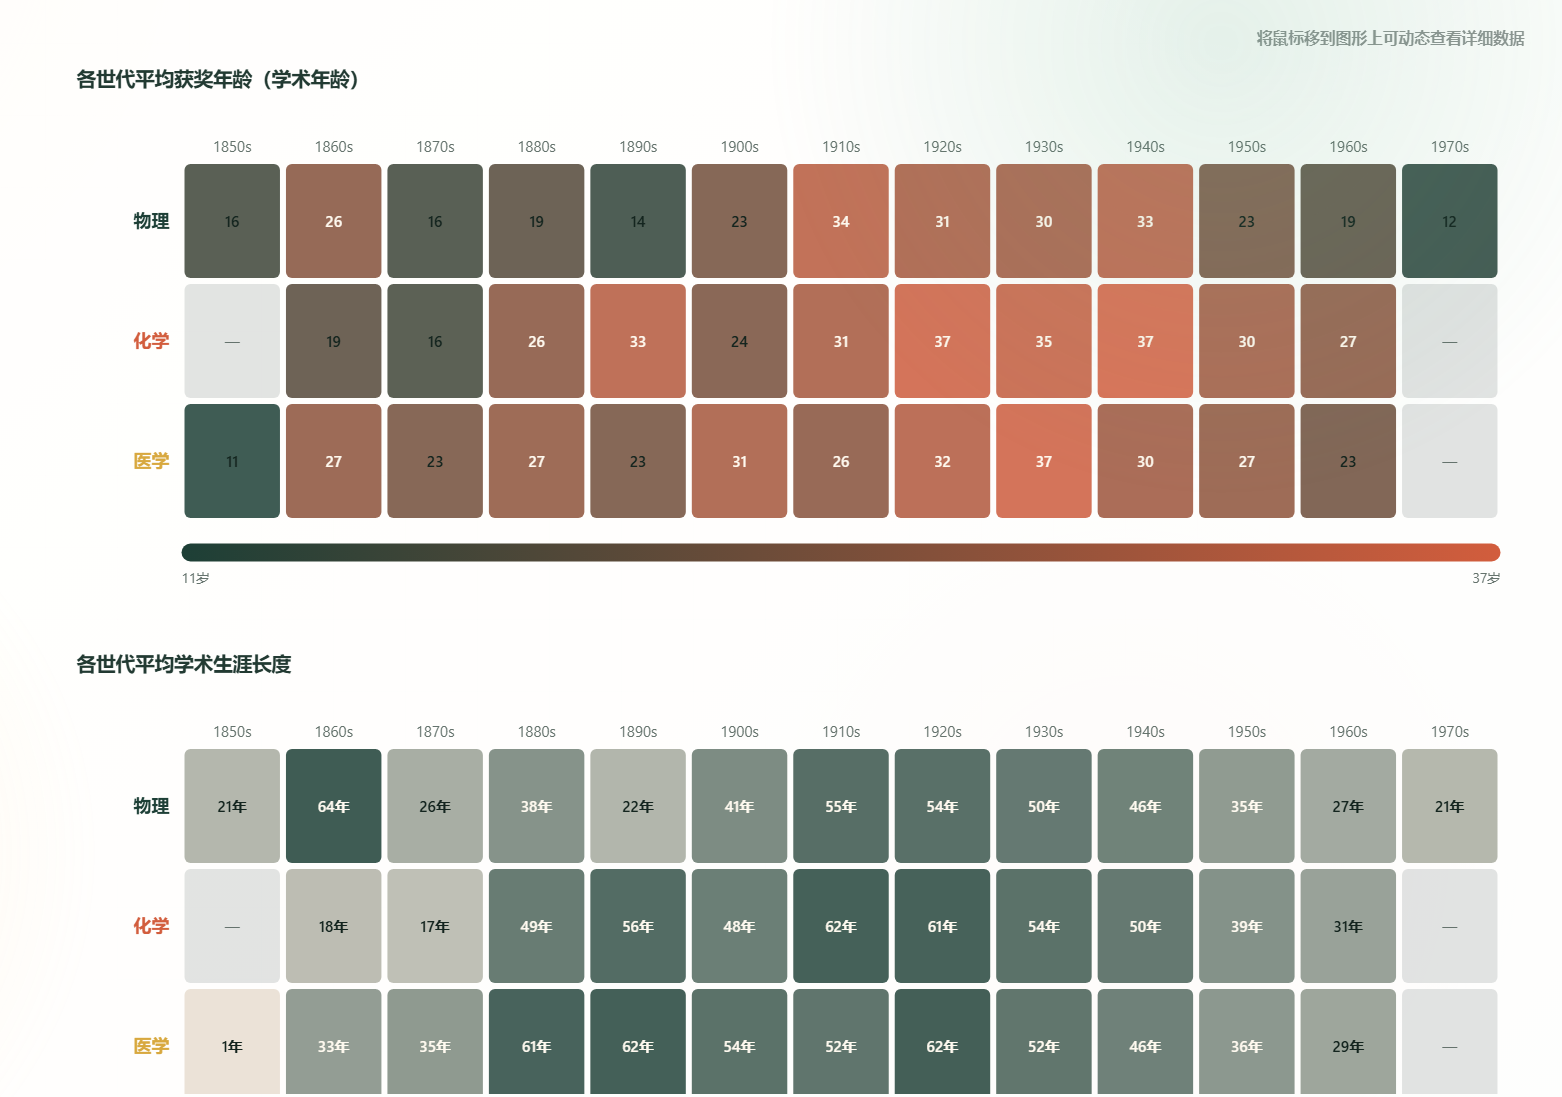
\includegraphics[width=\linewidth]{moduleB_cohort.png}
    \caption{出生世代比较（cohort 视图）}
    \label{fig:moduleB_cohort}
\end{figure}

\subsubsection{视图七：高产与低产个人的雷达对比（radar）}
该视图使用雷达图与散点图组合，从"论文总数""代表作被引""最高被引论文""产出持续时间""合作者数量""获奖时年龄"等多个维度对比高产得主与低产得主的特征分布。\autoref{fig:moduleB_radar}展示了这一视图。

雷达图显示高产得主在各维度上更饱满、均匀，尤其在"产出持续时间"和"合作者数量"上显著优于低产得主；右侧散点图进一步揭示，低产得主在"最高被引论文"这一维度上偶尔也能达到与高产得主相当的水平。这说明通往诺奖存在多种路径：部分得主靠持续的大量产出站稳脚跟，部分得主则凭借极少数高影响力的"天才之作"跻身诺奖殿堂。

\begin{figure}[H]
    \centering
    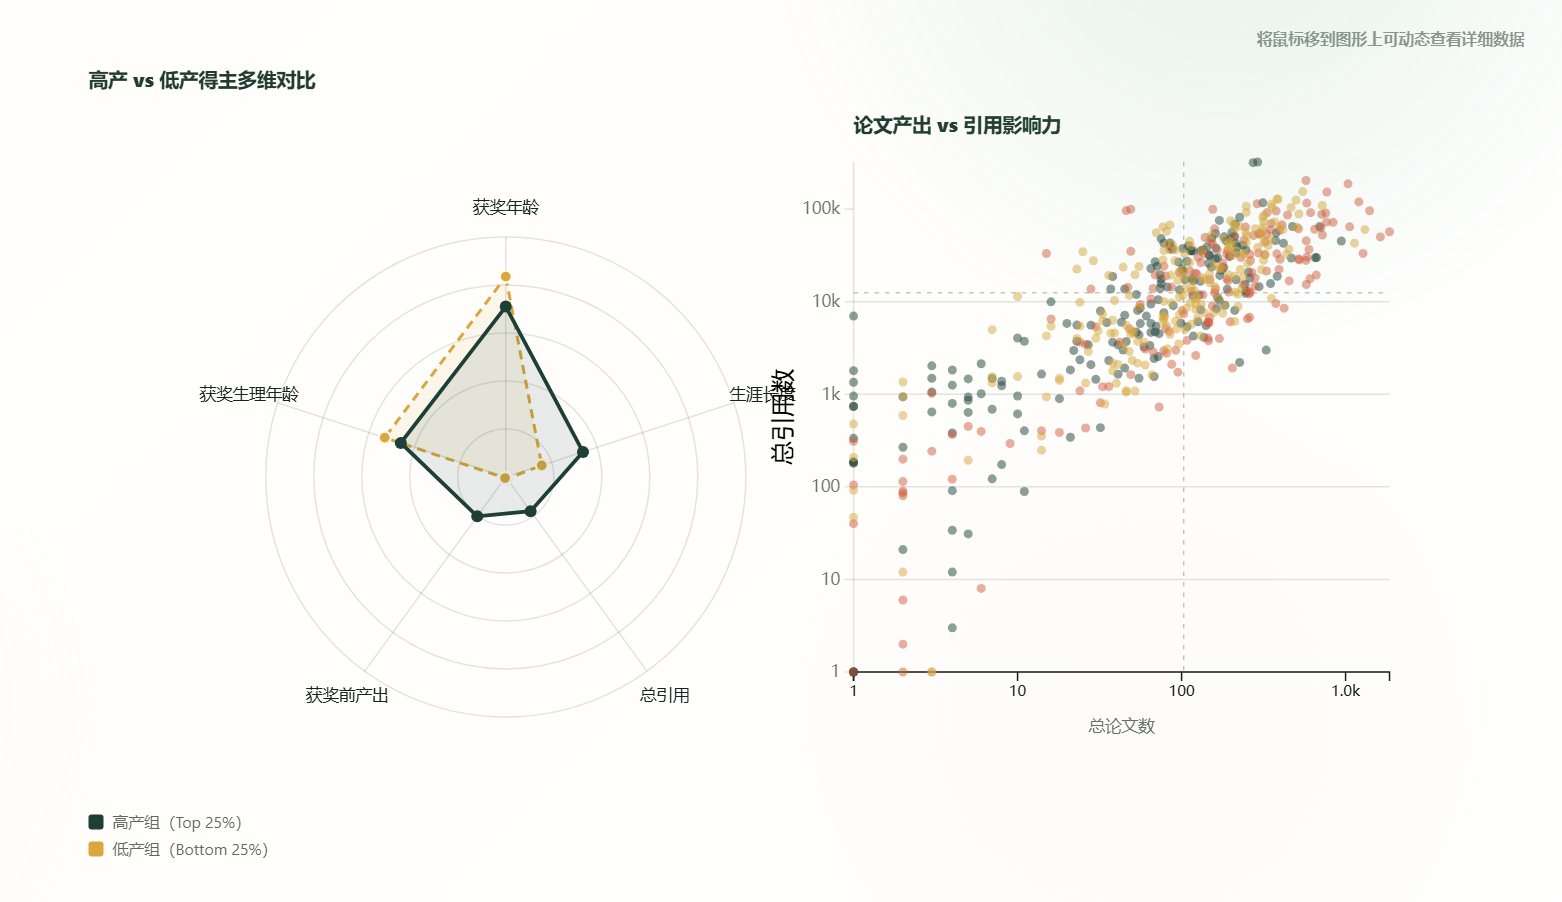
\includegraphics[width=\linewidth]{moduleB_radar.png}
    \caption{高产与低产得主的多维雷达对比（radar 视图）}
    \label{fig:moduleB_radar}
\end{figure}

\subsubsection{主要发现}
\begin{enumerate}
    \item \textbf{黄金创作窗口与"峰-奖错位"}：以首篇论文发表为原点，诺奖得主的平均产出高峰与平均获奖时间均出现在T+28左右，平均学术生涯跨度约48年。这意味着从学术生涯启动到获得诺奖认可，通常需要近三十年的持续积累。不同学科节奏各异：化学得主在T+28时的年均产出最高（约7.1篇），而物理与医学相对较低。
    \item \textbf{学科差异明显}：物理学得主的产出集中度显著高于医学，呈现更明显的单峰爆发特征；医学类得主则更多展现低集中度、长周期的平缓产出模式。不同学科的科研范式深刻影响了诺奖得主的学术生命周期。
    \item \textbf{世代变迁中的制度化趋势}：越晚出生的世代，从首篇论文发表到获奖的间隔越长（物理学科从1880s的16年延长至1930s的34年），且平均论文产出总量递增。现代诺奖越来越依赖长期积累与团队支持，个人天才叙事正在被制度化科研所改写。
    \item \textbf{多元路径}：高产与低产得主的雷达图及散点图对比表明，通往诺奖没有单一路线——持续的大量产出与少数高影响力的"天才之作"均可能通向斯德哥尔摩。低产得主在最高被引论文维度上偶尔可与高产者比肩，说明代表作质量与产出数量并非简单线性相关。
\end{enumerate}

\subsection{模块C：合作网络与内部引用（负责人：谷帅志）}

\subsubsection{设计目标}
模块 C 关注诺奖得主之间的合作关系与引用关系，回答"得主之间的合作和引用如何连接知识共同体"。模块基于D3.js 的小提琴图、弧线图与热力图组合，从三个递进的视角观察：团队规模如何演化、哪些得主之间存在合作弧线、内部引用网络具有怎样的结构。

\subsubsection{视图一：团队规模演化}
该视图以小提琴图（Violin Plot）呈现不同获奖年代诺奖论文的作者人数分布与演化趋势。\autoref{fig:moduleC_team_size}展示了这一视图。

横轴为获奖年代（1900–2010），纵轴为单篇论文作者人数。每个小提琴形状反映该年代作者数的分布密度，红色虚线标示中位数，蓝色虚线标示均值。用户可通过上方的学科筛选下拉框，分别查看物理、化学、医学三个子领域的趋势。视图的核心发现是：20世纪上半叶诺奖论文以单人作者或2–3人合作团队为主（中位数约1–2人）；1970年代以后，大团队协作成为常态，中位数逐步攀升；医学领域尤为突出——部分论文的作者人数超过100人（如大规模临床试验和多中心研究）。这一趋势直接反映了"大科学"时代科研组织方式的根本转变。

\begin{figure}[H]
    \centering
    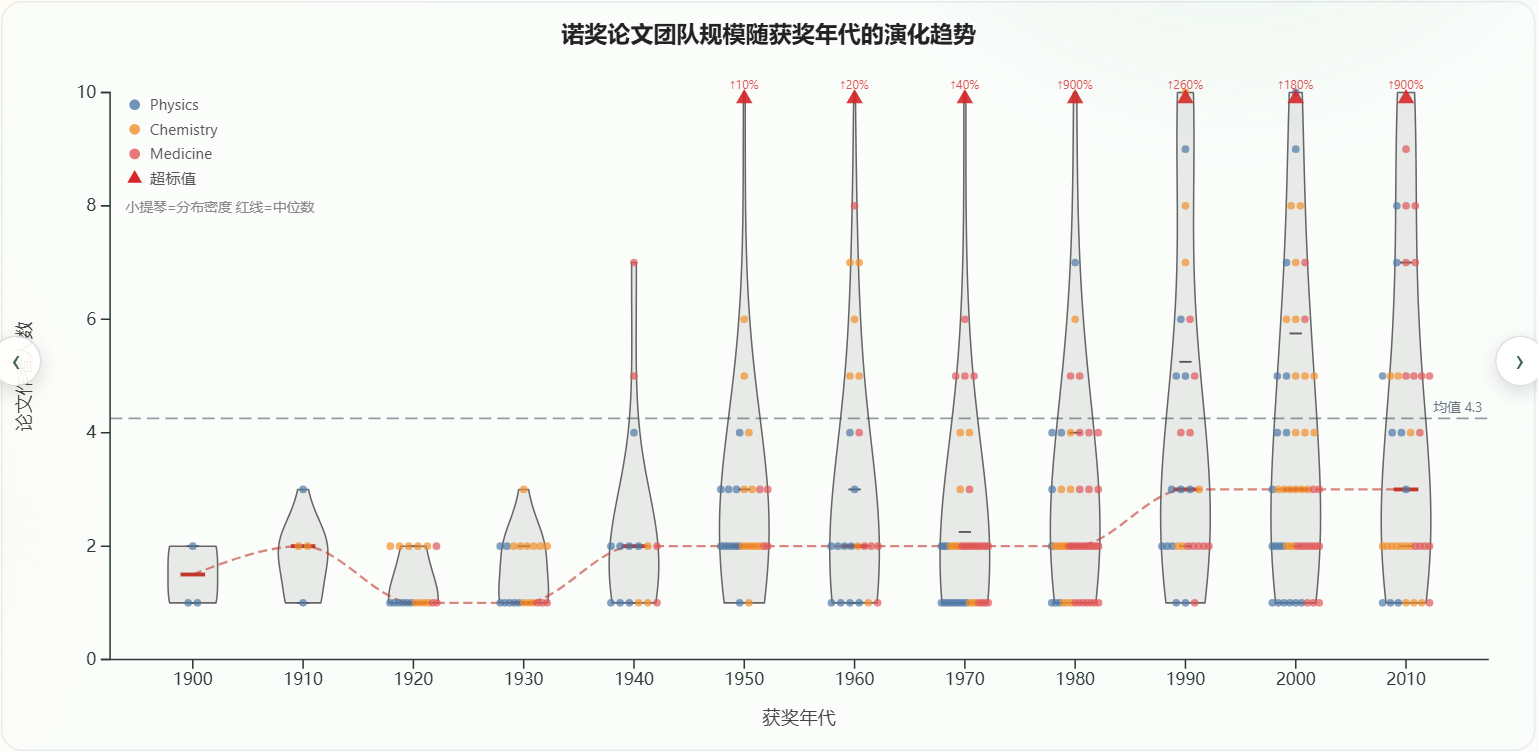
\includegraphics[width=\linewidth]{moduleC_team_size.png}
    \caption{团队规模演化：诺奖论文作者数量随时代增长}
    \label{fig:moduleC_team_size}
\end{figure}

\subsubsection{视图二：得主合作弧线}
该视图以弧线图（Arc Diagram）展示诺奖得主之间合著论文的频次。\autoref{fig:moduleC_collab_arcs}展示了这一视图。

沿着水平轴线排列着不同的诺奖得主姓名，连接任意两位得主的弧线表示他们曾在一篇或多篇论文中合作。弧线的粗细映射合作论文的数量；节点的颜色表示所属学科（物理、化学、医学）。用户可以通过控件设定"最低合作次数"和"显示最多关系条数"来调整网络的稠密度。视图揭示：物理学与化学之间跨学科的合著弧线最为密集（如玻尔与多位物理学家的合作），而医学得主间的合作弧线往往限于学科内部。少数"超级连接者"（如居里家族、玻尔、鲍林等）同时与多个子领域的多位得主存在合作，在网络中占据枢纽位置。

\begin{figure}[H]
    \centering
    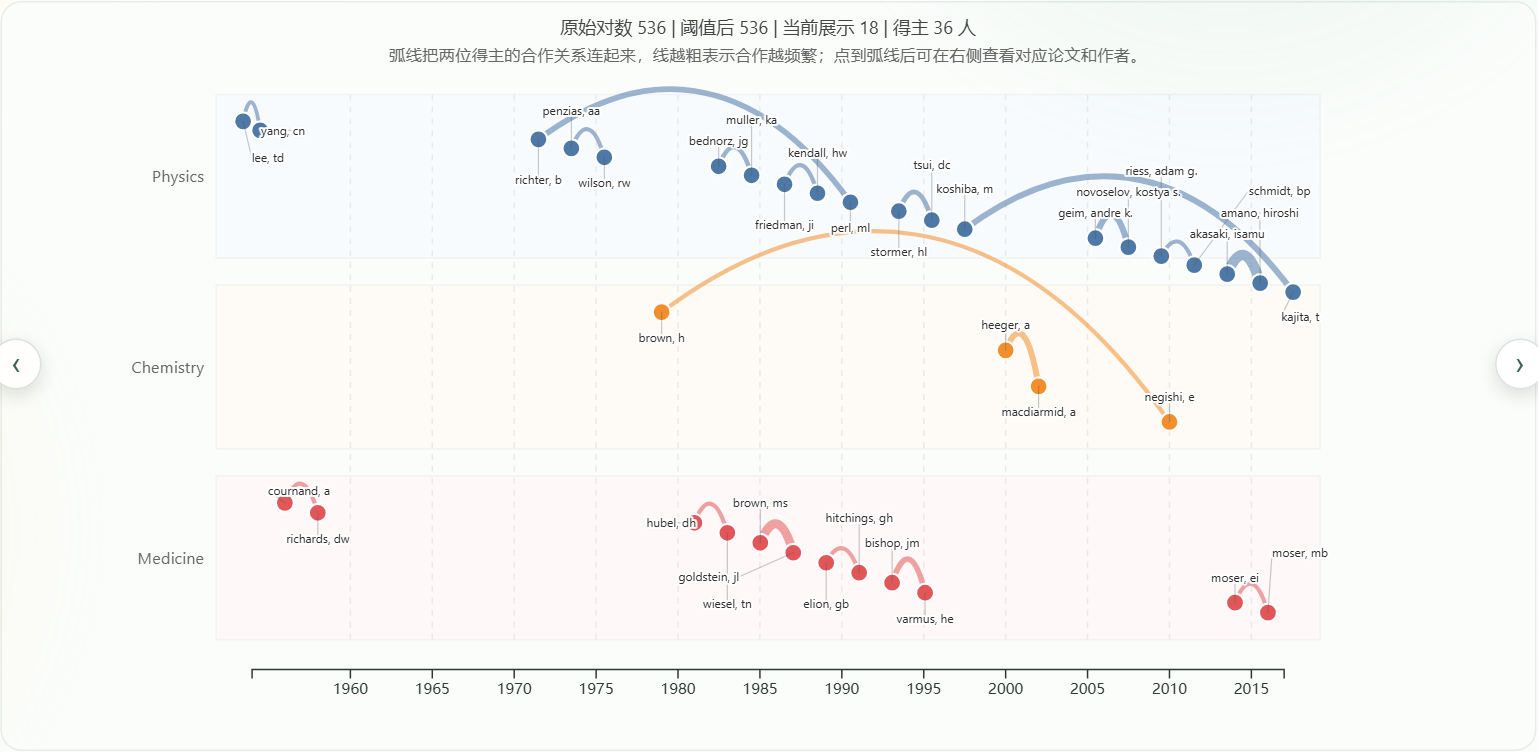
\includegraphics[width=\linewidth]{moduleC_collab_arcs.png}
    \caption{得主合作弧线：主要得主之间的合作频率}
    \label{fig:moduleC_collab_arcs}
\end{figure}

\subsubsection{视图三：内部引用热力}
该视图以热力图（Heatmap）展示不同诺奖得主之间的跨时引用结构。\autoref{fig:moduleC_citation_heat}展示了这一视图。

纵轴为被引论文的发表年份（1885–2015），横轴为引用论文的发表年份（1905–2015），每个单元格的颜色深度表示特定年份组合下的引用论文数量。用户可以通过学科筛选和聚合粒度控制(年份/五年/十年)来调节细度。视图的可选交互(如按引用关系类型聚类)揭示了:同一学科的得主之间引用密集,形成学科内的"引用小团体";但物理与化学之间存在显著的跨学科引用带,这与模块D 中"主题跨界"的发现相呼应。引用网络中的少数论文(如Watson \& Crick 的DNA 双螺旋、Einstein 的广义相对论等)形成了跨越多个学科和世代的引用高峰。

\begin{figure}[H]
    \centering
    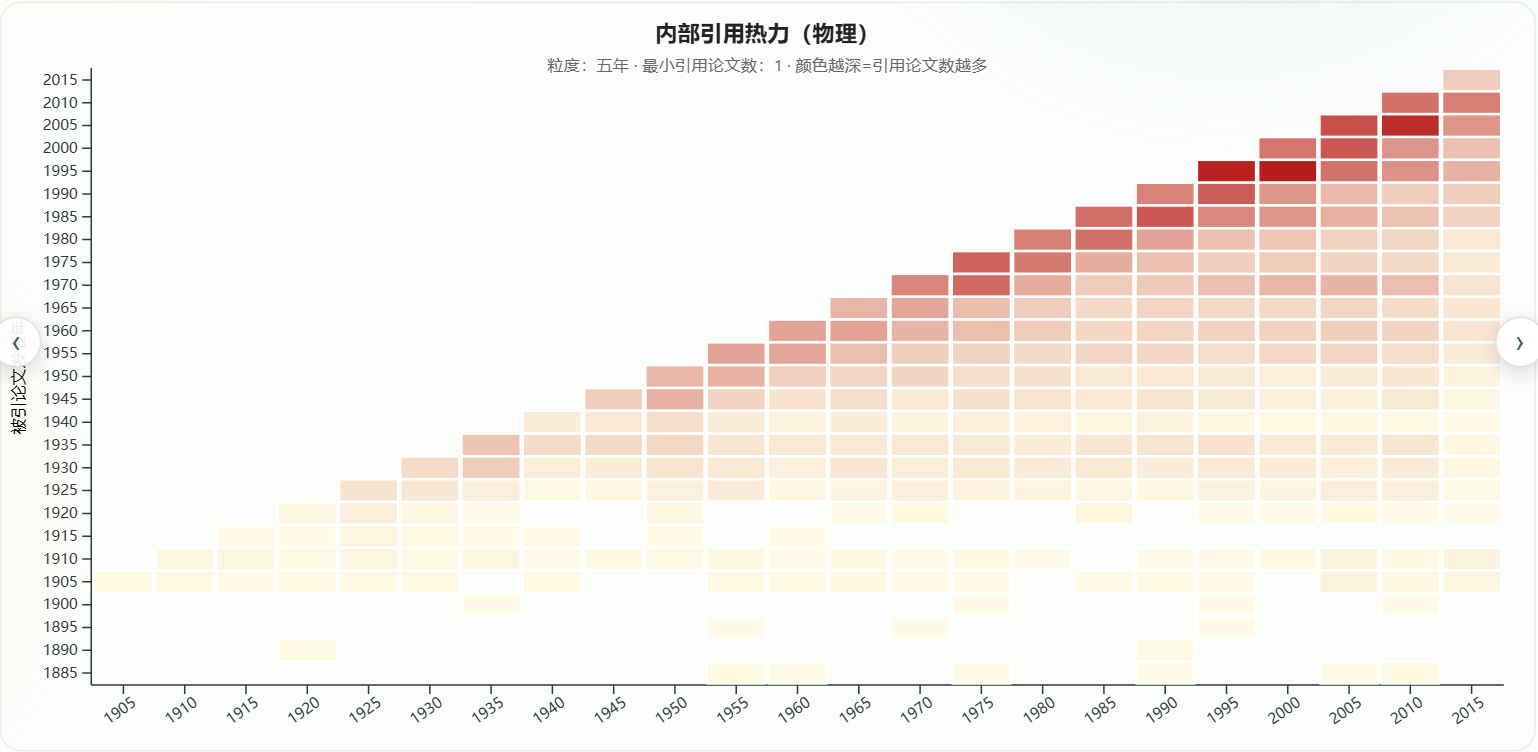
\includegraphics[width=\linewidth]{moduleC_citation_heat.png}
    \caption{内部引用热力：得主之间的引用密度分布}
    \label{fig:moduleC_citation_heat}
\end{figure}

\subsubsection{主要发现}
\begin{enumerate}
    \item \textbf{合作密度随时代明显上升}：20 世纪下半叶以来，诺奖论文的合作者数量显著增加，从单人作者到数十人甚至上百人团队，反映了"大科学"时代科研范式的根本转变。医学领域的团队化程度最高，这与临床试验和多中心研究的组织方式密切相关。
    \item \textbf{跨学科合作是诺奖级突破的重要特征}：图16中，物理学与化学、物理与医学之间的跨学科合著弧线虽数量有限，但连接了不同领域的核心节点；结合图17的跨时引用热力可见，早期奠基性论文在数十年间持续被多学科引用，形成知识共同体的核心纽带。许多重大诺奖成果（如放射性研究、DNA结构解析、集成电路发明等）都诞生于学科交叉地带。
    \item \textbf{少数超级连接者}：少数得主作为"超级连接者"在历史合作与引用网络中占据核心位置。图16 所示的近期合作网络中，连接多个子领域的多节点枢纽延续了这一模式，将不同领域紧密连接成知识共同体，体现了科研"传承"在诺奖故事中的重要作用。
\end{enumerate}

\subsection{模块D：研究主题的迁移与跨界（负责人：张帅康）}

\subsubsection{设计目标}
模块 D 从 OpenAlex 提供的微观主题（Subfield 层级）出发，追踪诺奖论文的研究主题如何随年代更替而迁移、如何跨越传统学科边界，以及不同得主在主题覆盖范围上的差异。模块以桑基图（Alluvial Diagram）为核心，辅以学科跨界矩阵和得主扩散度分布。

\subsubsection{视图一：主题随时代演化（evolution）}
该视图以堆叠面积图（Streamgraph）形式，展示不同年代（1900s–2010s）诺奖论文的OpenAlex主题分类占比演化。\autoref{fig:moduleD_evolution}展示了这一视图（以医学奖为例）。

各层面积代表具体主题（如"Nitric Oxide and Endothe..." "Growth Hormone and Insul..." "RNA and protein synthesis..."等），面积高度表示该主题在特定年代的论文记录占比。颜色按主题着色。从图中可清晰看到：20世纪早期医学奖论文集中于"RNA and protein synthesis..."等基础生物化学主题；1930–1950年代"Growth Hormone and Insul..."占比达到峰值；1970–1990年代"Prion Diseases and Prote..."与"Neuroscience and Neuroph..."逐步扩张；21世纪"Cellular transport and s..."与神经科学相关主题成为占比最高的领域。用户可通过顶部筛选器切换学科（物理/化学/医学）和观察窗口（1900年以来/1900–1949/1950–1989/1990–2019），观察不同学科的演化节奏差异。

\begin{figure}[H]
    \centering
    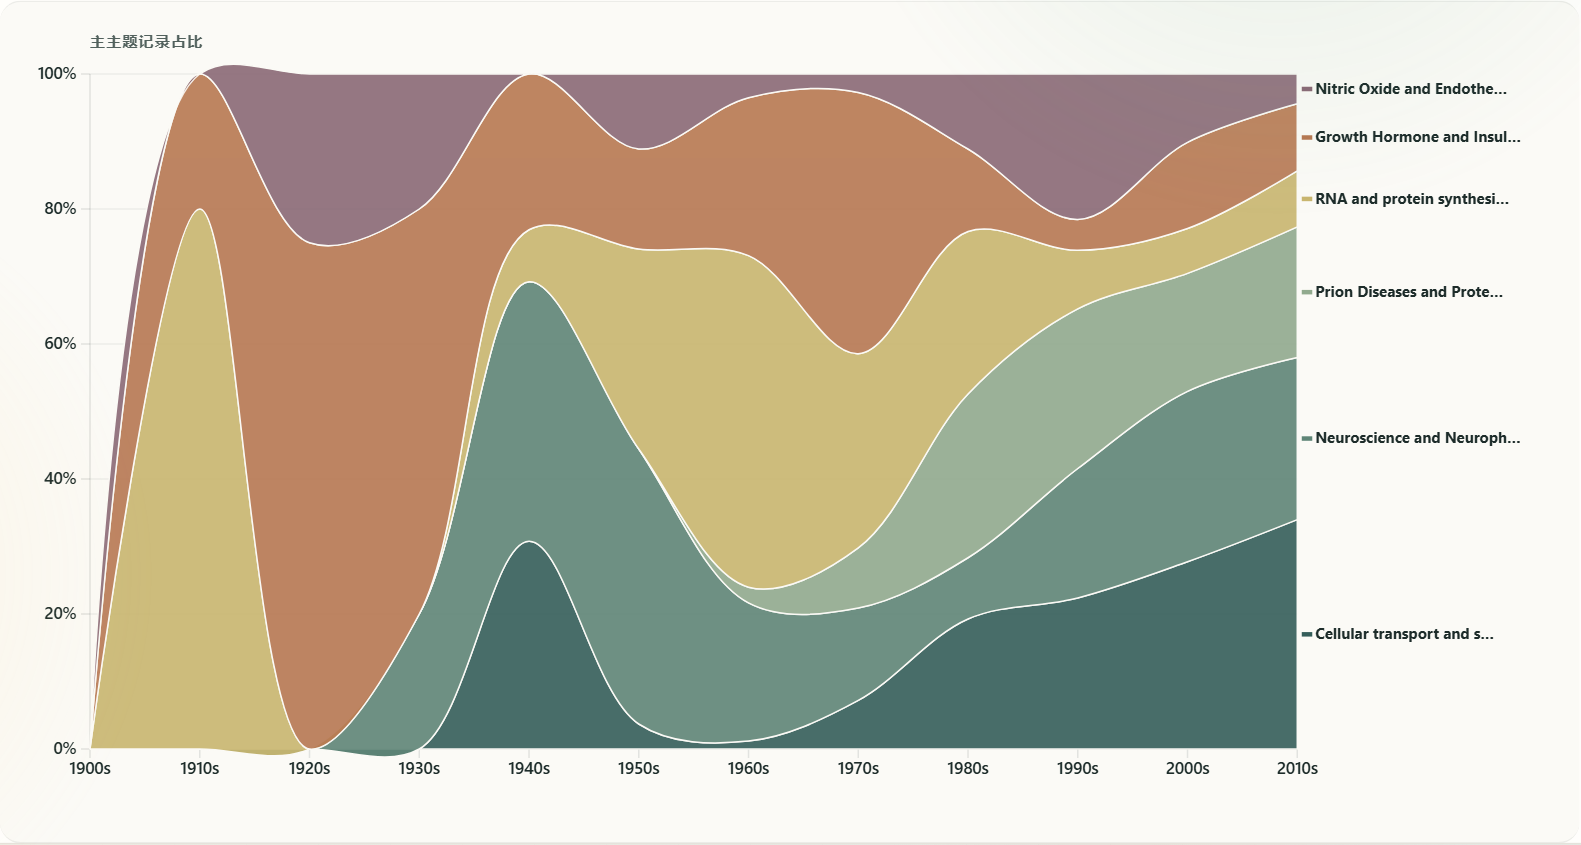
\includegraphics[width=\linewidth]{moduleD_evolution.png}
    \caption{主题随时代演化：Alluvial 主题迁移流}
    \label{fig:moduleD_evolution}
\end{figure}

\subsubsection{视图二：学科破壁（bridges）}
该视图以桑基图（Sankey Diagram）形式，量化展示来自不同传统学科的论文在主题层面上的交叉归属情况。\autoref{fig:moduleD_bridges}展示了这一视图。

左侧为传统诺奖类别（物理、化学、医学），右侧为OpenAlex微观主题，流线的宽度表示属于左侧学科分类的论文被归入右侧主题分类的数量。从流线分布可见，物理、化学、医学各自向本学科主题输出的流量最大，但跨学科流同样显著。这反映了分子生物学、纳米科学、量子生物学等跨学科领域的兴起正在模糊传统学科边界。

\begin{figure}[H]
    \centering
    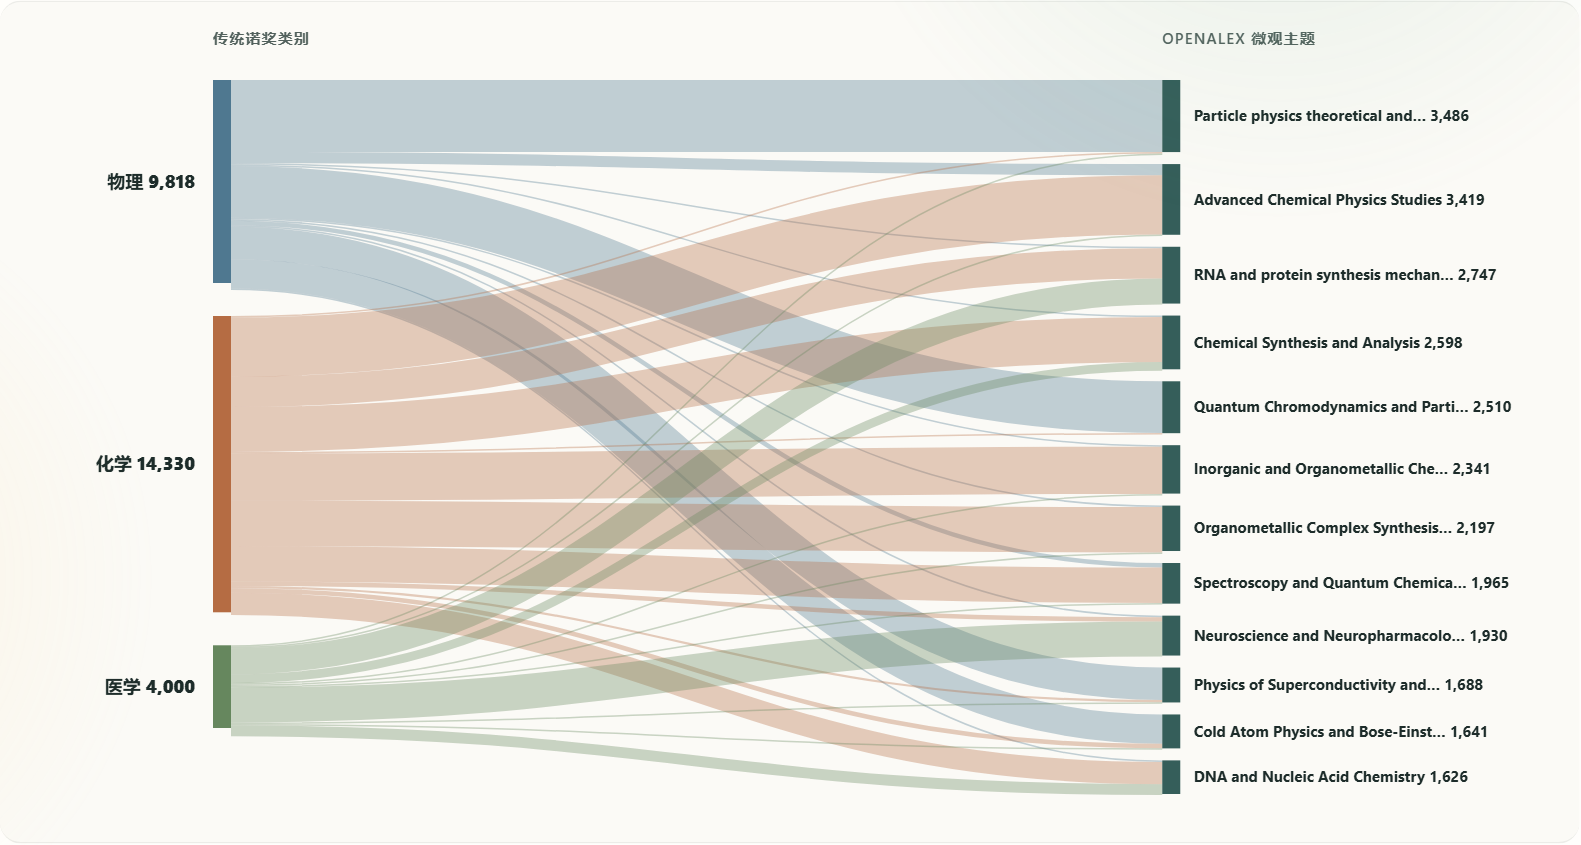
\includegraphics[width=\linewidth]{moduleD_bridges.png}
    \caption{学科破壁：主题跨越传统学科边界的频度}
    \label{fig:moduleD_bridges}
\end{figure}

\subsubsection{视图三：得主扩散度（breadth）}
该视图以散点图（气泡图）展示每位诺奖得主论文在OpenAlex主题分类中的覆盖广度与集中度的关系。\autoref{fig:moduleD_breadth}展示了这一视图。

每个气泡代表一位得主，横轴为论文数量与主题记录数量的比值（对数轴），纵轴为主题扩散指数；气泡面积映射其累计主题标注数量，颜色深浅表示Top 10\%论文占比。图中清晰显示：大多数得主聚集在左上方（少量论文但主题分散，扩散指数高于0.8），而右下角有少数高产且主题相对集中的得主（如Omura、Schally等）。标注于右上方的高产且跨域得主（如Edelman、Baltimore、Roberts）呈现多面手特质。整体而言，得主在主题覆盖策略上存在显著个体差异——部分深耕单一领域，部分则在多个领域产出影响深远的成果，两种路径都能通往斯德哥尔摩。


\begin{figure}[H]
    \centering
    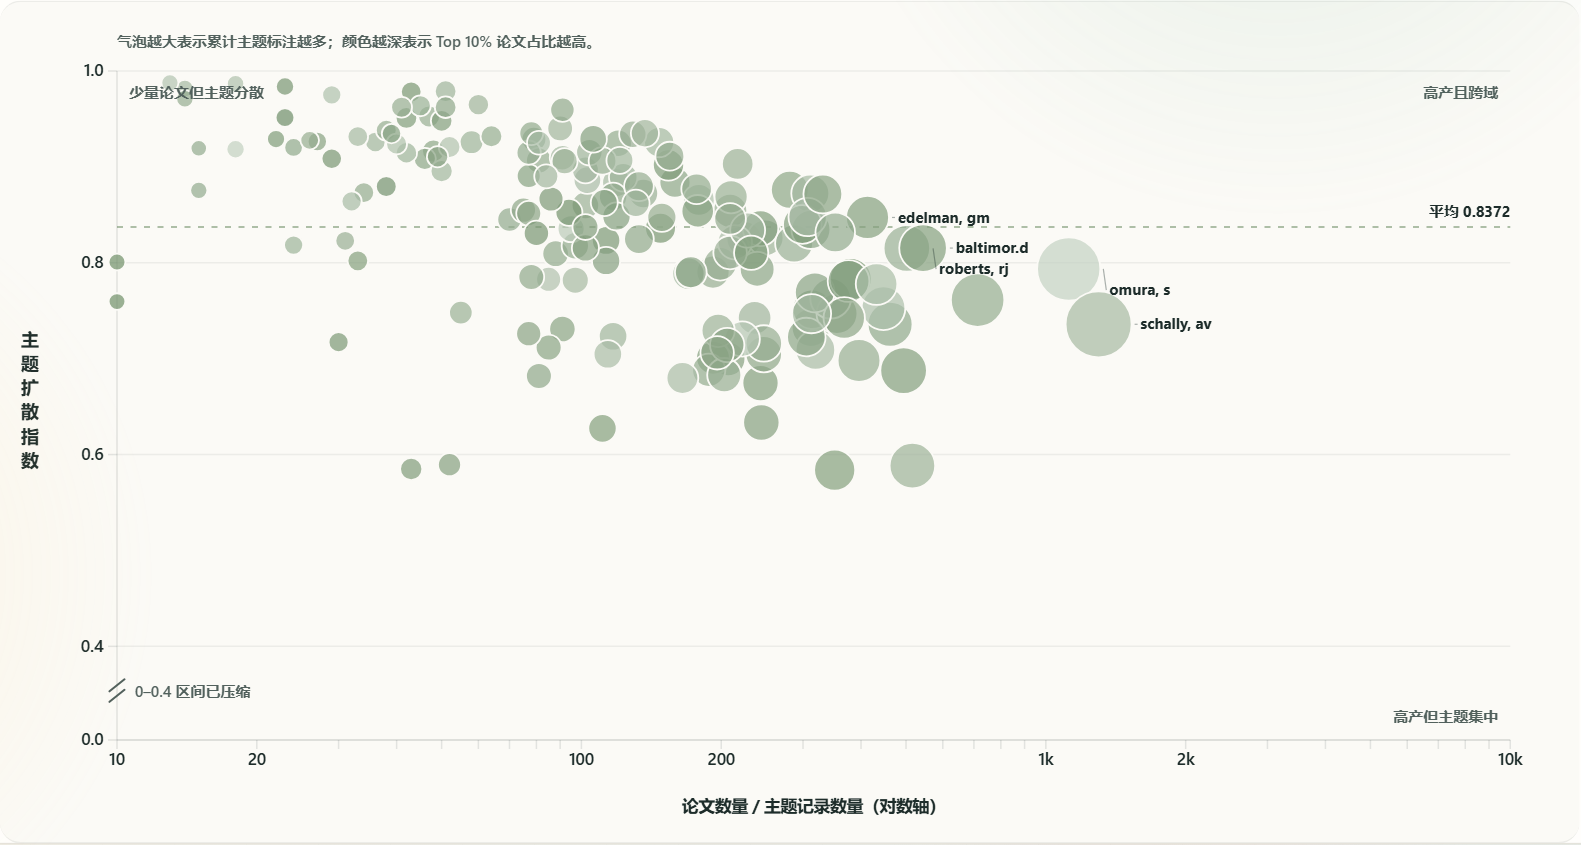
\includegraphics[width=\linewidth]{moduleD_breadth.png}
    \caption{得主扩散度分布：主题覆盖的广度与集中度}
    \label{fig:moduleD_breadth}
\end{figure}

\subsubsection{主要发现}
\begin{enumerate}
    \item \textbf{学科细化}：20 世纪以来，诺奖研究主题从早期相对单一的分类（如"光学""热力学""有机化学"）逐渐细化为数十个子领域。从桑基图中的流动可以看到，高分子化学、分子生物学、量子信息等新兴子领域在 1960 年代以后陆续从母学科中分化出来。
    \item \textbf{跨界突破}：许多重大诺奖成果（如 DNA 双螺旋、CRISPR 基因编辑、引力波探测等）都源自物理学、化学与生物学的深度融合。学科破壁矩阵证实了这种跨界趋势在 21 世纪后显著加剧，跨学科交叉已经不再是例外，而是诺奖级标准配置。
    \item \textbf{主题扩散的多样性}：得主扩散度散点图揭示，诺奖得主在研究广度上存在显著个体差异。部分得主一生深耕单一主题，凭借极深的专业造诣摘得诺奖；另一些得主则在多个领域产出影响深远的成果。两种路径都能通往斯德哥尔摩，但跨学科覆盖广度在21世纪后变得更具竞争力。
\end{enumerate}

\subsection{模块E：代表作长尾影响力（负责人：游子力）}

\subsubsection{设计目标}
模块 E 聚焦于诺奖得主代表作的被引分布，回答"代表作为什么能从浩如烟海的论文中凸显出来"。模块以 Log-Log 坐标下的被引散点图、动态筛选面板和分学科对比为核心手段，揭示长尾影响力的形成机制。

\subsubsection{视图设计：学科视角下的代表作影响力散点图}
由于模块 E 以单视图交互为核心（通过 tab 切换物理/化学/医学三个学科视角），此处一并展示模 E 统一布局下的三个学科截图。\autoref{fig:moduleE_medicine}、\autoref{fig:moduleE_physics}、\autoref{fig:moduleE_chemistry}分别展示了医学、物理、化学三个学科的代表作长尾分布。

该视图使用 Log-Log 散点图，横轴为论文被引次数的秩次排名，纵轴为对应的被引次数。每个点代表一篇诺奖得主的代表作，点的大小映射 FWCI（Field-Weighted Citation Impact），颜色深浅表示论文发表年代。左侧的筛选面板允许用户调节最小 FWCI 阈值和最小引用数阈值，动态过滤底层数据。随着阈值提高，少数位于散点图右上角（高秩次与高被引量）的论文被突出显示。

在医学视角中，Watson \& Crick 的DNA 双螺旋论文（1953年，被引约7,000次）在长尾顶端的突出表现尤为醒目。物理学视角中，量子力学奠基性论文与凝聚态物理相关代表作占据长尾顶端。化学视角中，鲍林的化学键理论论文、高分子化学代表作以及近年来CRISPR基因编辑相关论文（被引约15,000次）持续位于被引前列。

\begin{figure}[H]
    \centering
    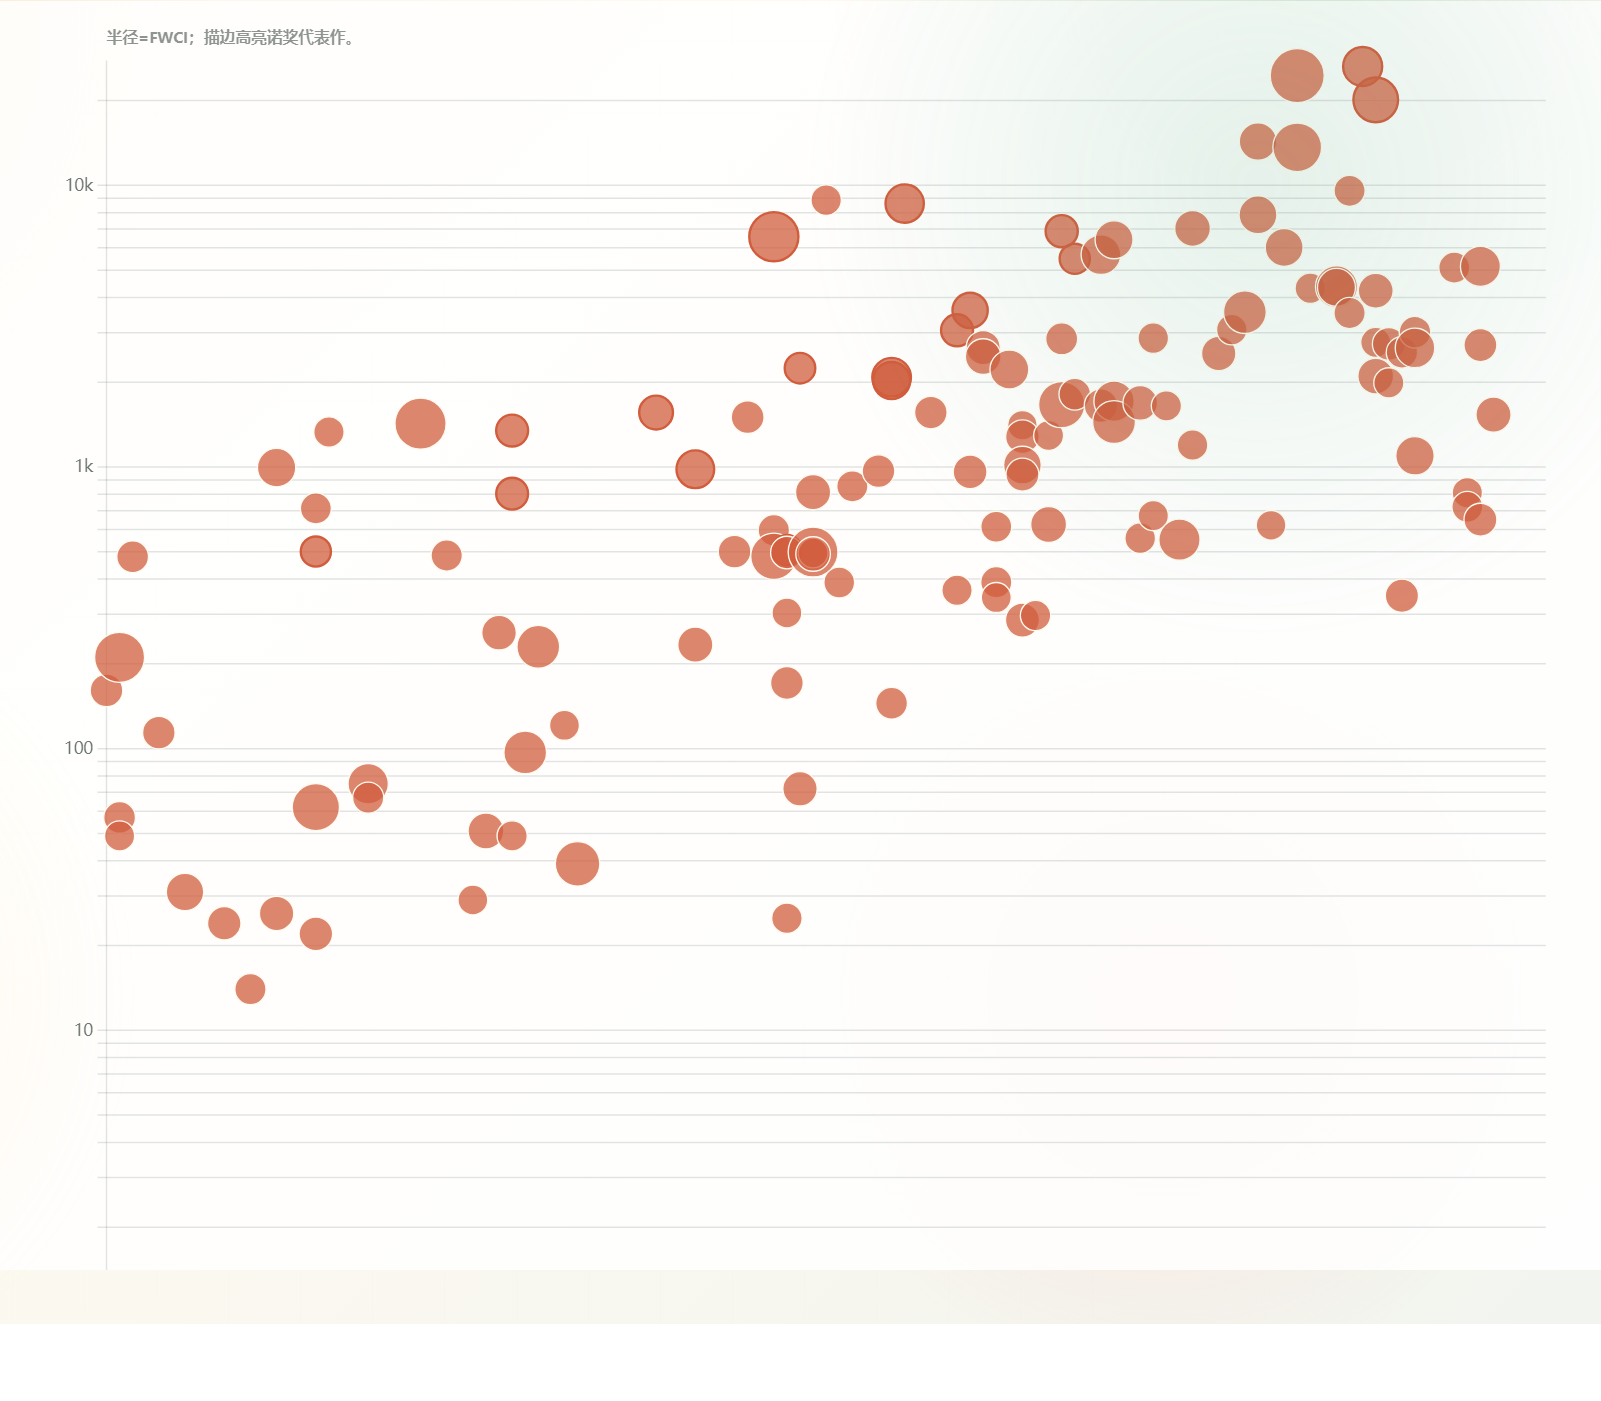
\includegraphics[width=\linewidth]{moduleE_medicine.png}
    \caption{代表作长尾影响力：生理学或医学领域}
    \label{fig:moduleE_medicine}
\end{figure}

\begin{figure}[H]
    \centering
    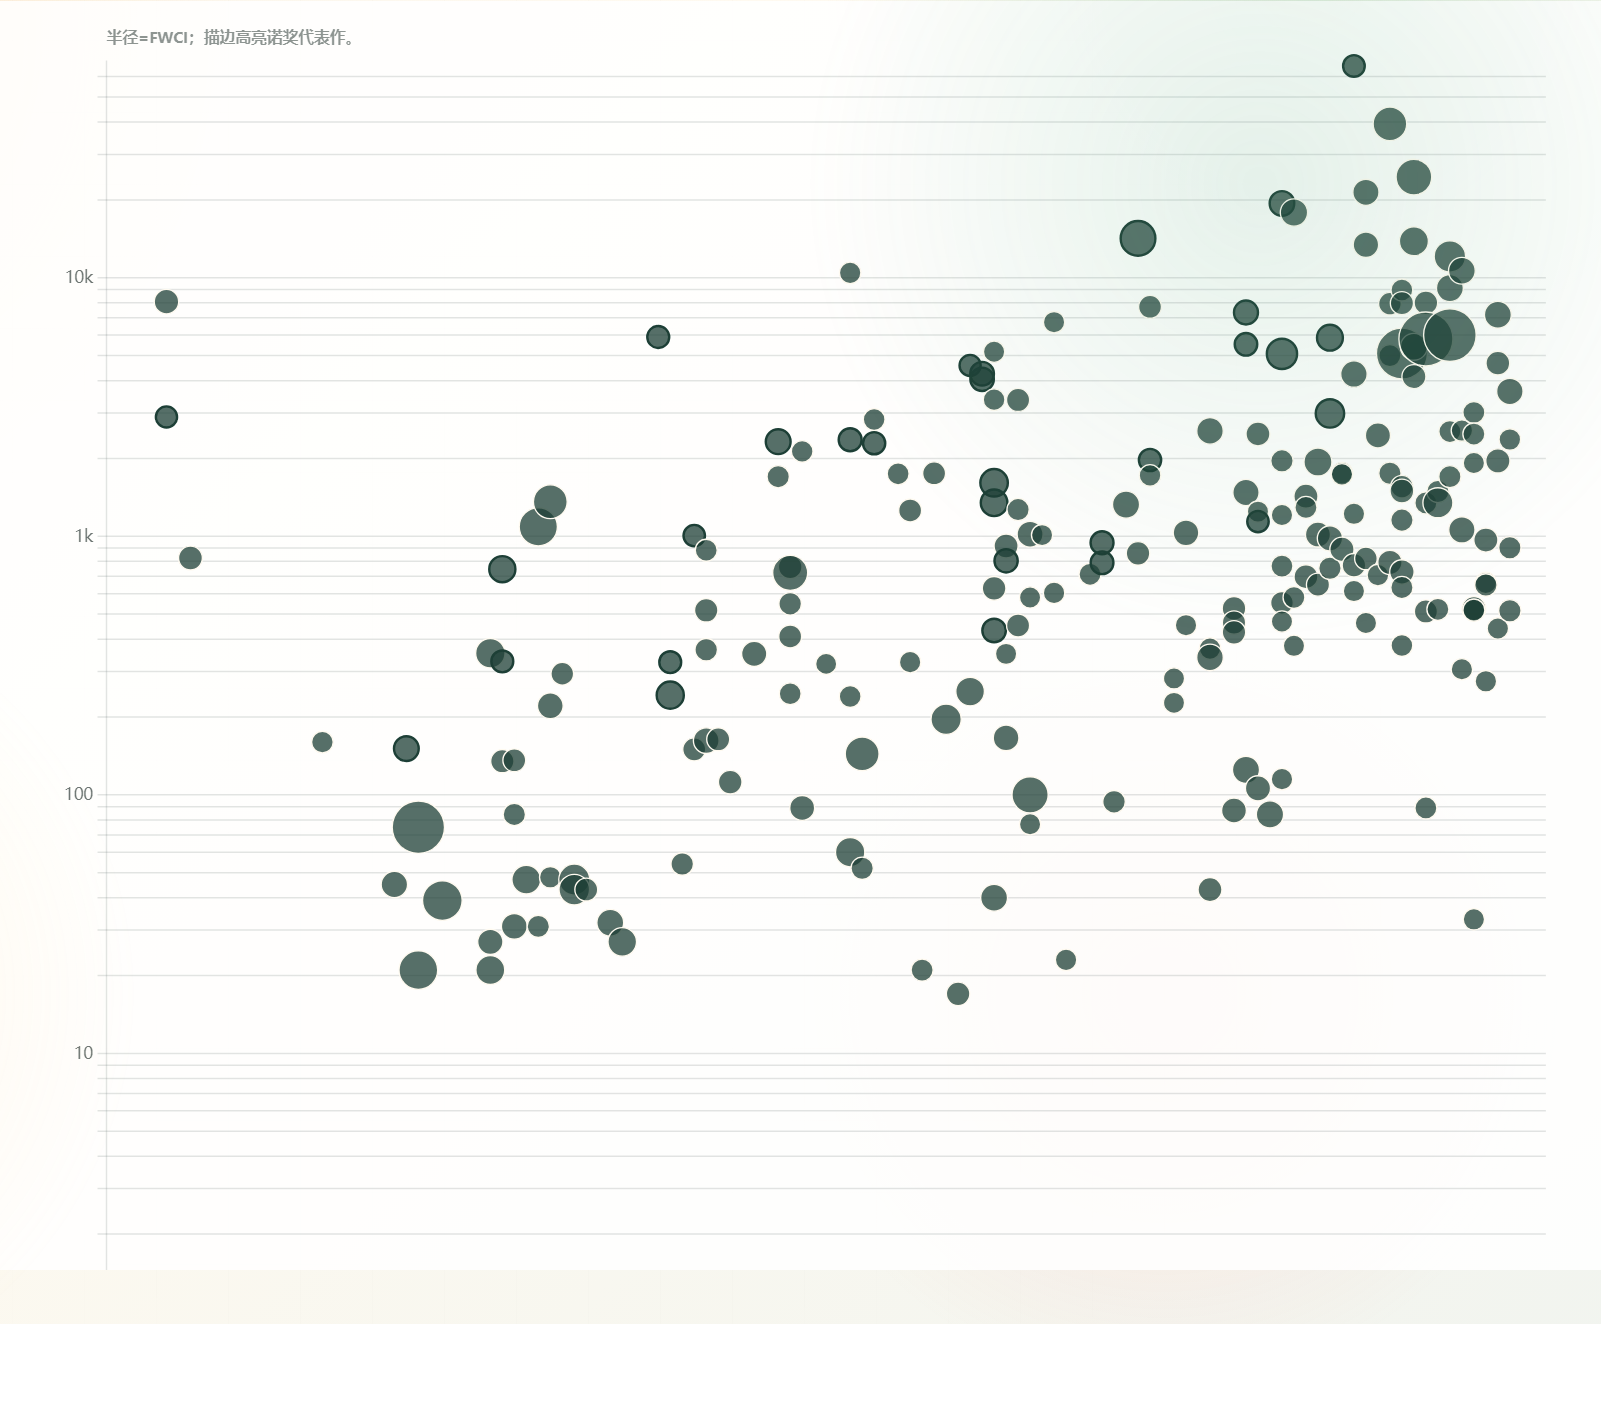
\includegraphics[width=\linewidth]{moduleE_physics.png}
    \caption{代表作长尾影响力：物理学领域}
    \label{fig:moduleE_physics}
\end{figure}

\begin{figure}[H]
    \centering
    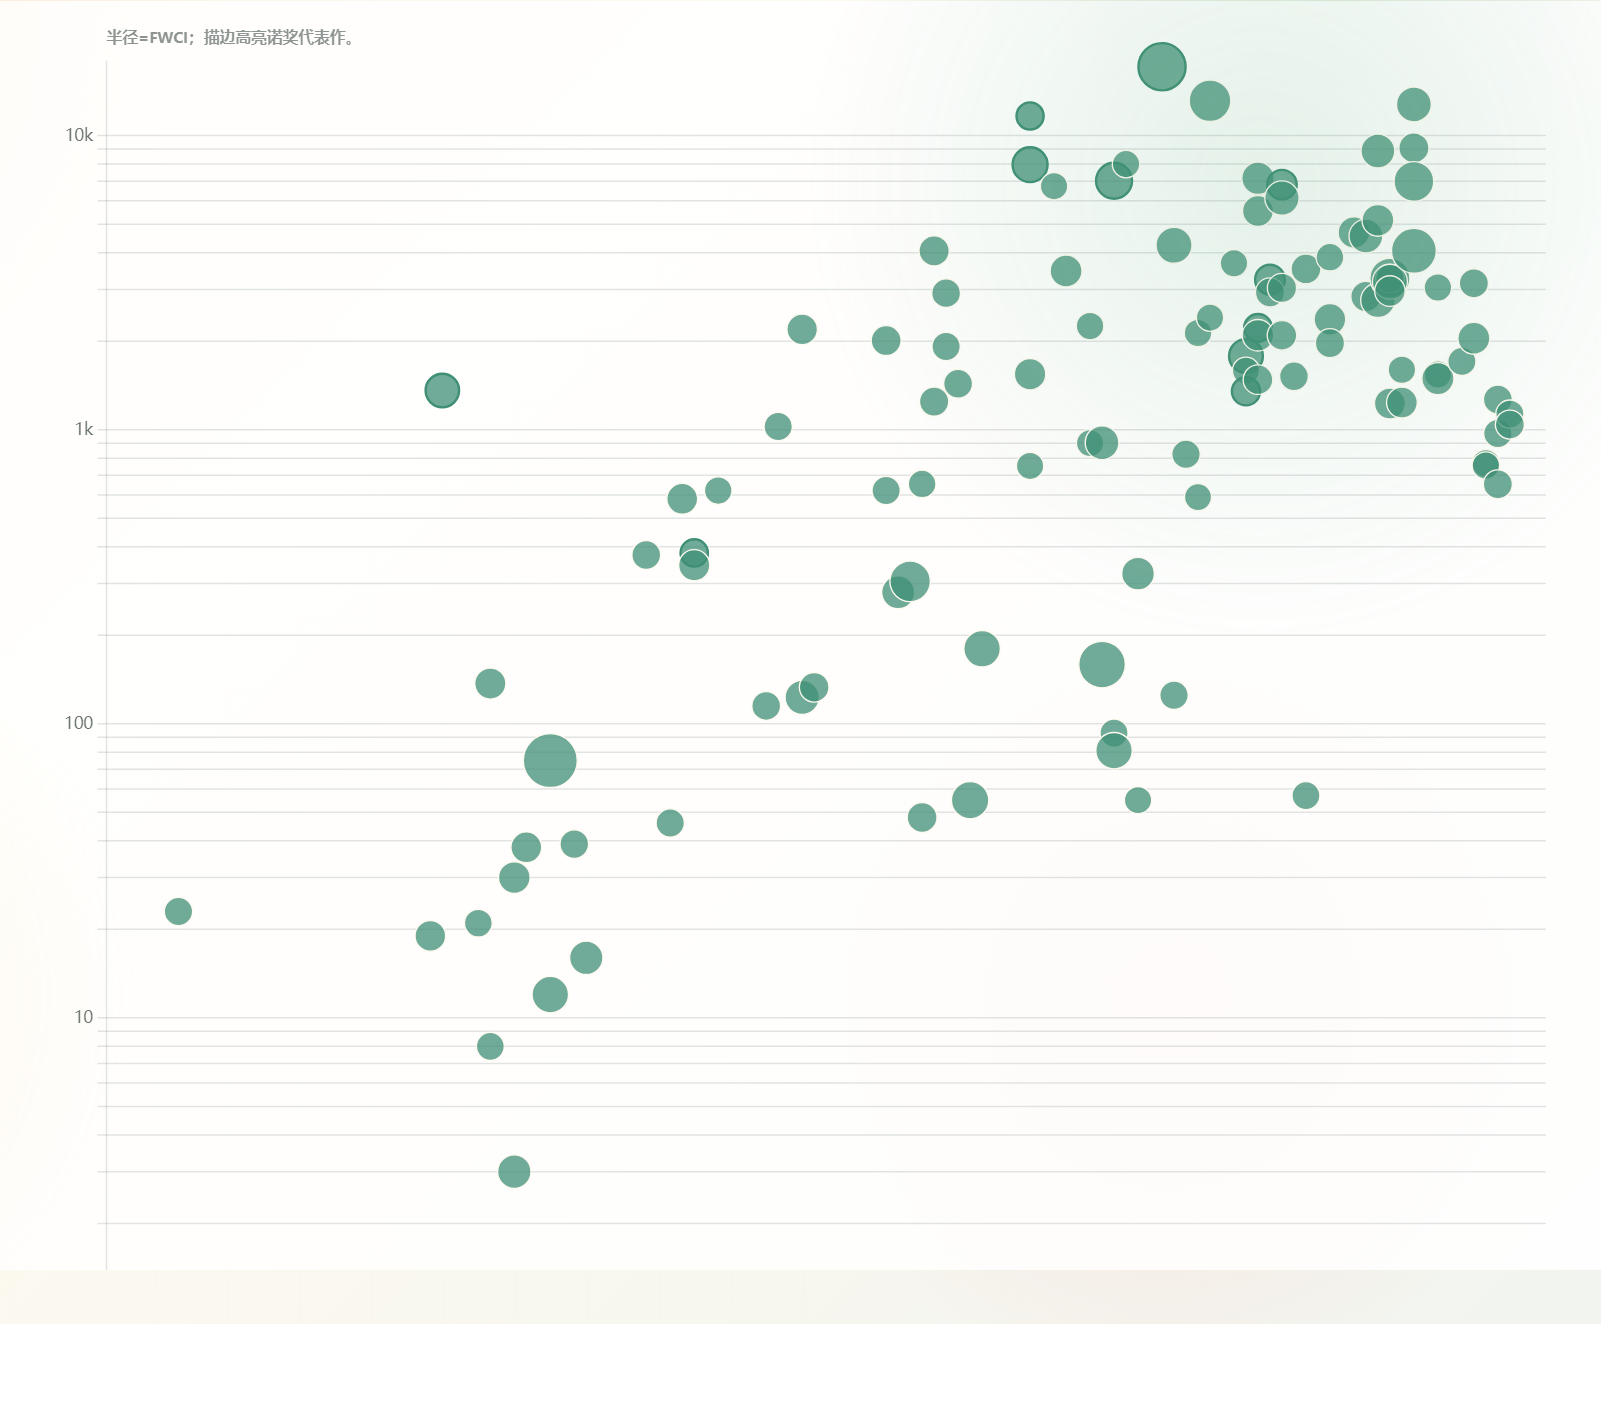
\includegraphics[width=\linewidth]{moduleE_chemistry.png}
    \caption{代表作长尾影响力：化学领域}
    \label{fig:moduleE_chemistry}
\end{figure}

\subsubsection{主要发现}
\begin{enumerate}
    \item \textbf{幂律分布显著}：诺奖代表作的被引频次在三个学科中均呈现明显的幂律分布（Power-law Distribution），即少数论文占据了引用总量的绝大部分。
    \item \textbf{时间累计优势}：发表年份较早的代表作（20世纪上半叶）往往在长尾顶端占据更稳固的位置。时间累积是长尾形成的最重要因素——论文发表越早，积累被引的时间窗口越长。但同时，少数近年发表的"当代经典"（如CRISPR相关论文）也展现了快速爬升的趋势。
\end{enumerate}

\section{总结与展望}
\subsection{核心结论}
本项目以"如何拿诺奖"为叙事主线，从空间、时间、关系、主题与影响力五个维度对诺贝尔奖得主的数据进行了整合与可视化。我们最终得知想要拿诺奖我们应该怎么做：\textbf{如果把诺奖看成一条路线，数据给出的提示很朴素：去高密度科学中心，抓住创作窗口，和重要的人一起解决重要的问题，敢于突破传统的主题，让成果在很久以后仍然被引用。}
而分别看五个模块的发现，我们得到以下五条核心结论：
\begin{enumerate}
    \item \textbf{空间——科学中心转移}：诺奖资源高度集中于少数国家和顶尖机构。20世纪早期欧洲占据主导地位，德国在1901–1938年间显著领先；二战后美国成为绝对主导的学术中心。21世纪以来日本等亚洲国家的诺奖得主数量显著上升，全球科学多极化趋势初显。
    \item \textbf{时间——“迟来的认可”}：诺奖代表作主要在获奖前完成，学术生涯中期（T+20至T+35）是"黄金创作窗口"。以首篇论文发表为原点，平均获奖时间约为T+28，代表作与获奖之间普遍存在数年乃至十余年的时间差。各年代得主的生理获奖年龄持续推迟（从1900年代的约50岁升至2020年代的65岁以上），现代诺奖越来越依赖长期积累，奖项在确认影响而非发现突破本身。
    \item \textbf{关系——合作的力量}：20世纪下半叶以来，诺奖论文的合作者数量显著增加，从单人作者发展到数十人乃至上百人的大团队，医学领域尤为突出。跨学科合作是诺奖级突破的重要特征，物理与化学、化学与医学之间的主题交叉持续深化。历史上少数"超级连接者"（如居里家族、玻尔、鲍林）曾将不同子领域连接成知识共同体，这一网络化的科研传统在当代合作模式中得以延续。
    \item \textbf{主题——持续的跨界与细化}：诺奖研究主题从早期相对单一的分类逐步细化为数十个微观子领域，且跨学科融合趋势在21世纪显著加速。物理、化学与医学之间的主题边界日益模糊，学科破壁已从例外变为常态。
    \item \textbf{影响——时间累积的长尾}：代表作被引呈幂律分布，发表时间越早的论文通常具有更大的累积优势。但少数近年发表的"当代经典"（如CRISPR相关论文）亦展现出快速爬升趋势。诺奖更像知识长期积累后的迸发，而非瞬间的灵感闪耀。
\end{enumerate}

\subsection{设计反思}
尽管项目在数据整合与可视化设计方面取得了一定成果，但仍存在以下不足：
\begin{enumerate}
    \item \textbf{数据覆盖}：本项目在深度分析中主要聚焦于物理、化学、生理医学与经济学四个科学奖项；文学奖与和平奖因论文数据特殊性未进入模块B–E的定量分析；
    \item \textbf{性别与少数群体}：模块未对诺奖得主的性别、族裔等维度进行单独分析，这些维度对理解诺奖公平性具有重要意义；
    \item \textbf{可访问性}：当前前端主要面向桌面浏览器优化，对移动端、屏幕阅读器等辅助技术的支持尚需加强；
    \item \textbf{交互深度}：部分图表目前仅支持基本的悬停提示和筛选操作，未来可考虑增加更丰富的钻取和故事线导览。
\end{enumerate}

\subsection{未来工作}
在后续工作中，我们计划从以下方向进一步推进：
\begin{enumerate}
    \item 引入更多数据源（如 Semantic Scholar、Crossref），扩展论文维度的指标体系；
    \item 增加性别、年龄、国别等维度的对比分析，提升项目的社会价值；
    \item 引入机器学习方法，对"诺奖潜力"进行建模预测，探索数据驱动的科研评估；
    \item 优化移动端适配与可访问性，使项目能够被更广泛的受众使用。
\end{enumerate}

\section{致谢}
本项目是北京大学信息管理系"数据可视化"课程的期末项目，由第 6 小组在 2026 年春季学期共同完成。在项目进行过程中，我们得到了授课老师与助教的悉心指导，也得到了课程平台对小组协作的支持。在此特别感谢小组六位成员在数据处理、可视化设计、前端开发与报告写作中的通力合作：陈湘媛（地缘政治与空间轨迹）、黎子游（学术生命周期）、谷帅志（合作网络与内部引用）、张帅康（研究主题迁移与跨界）、游子力（代表作长尾影响力）以及陈诣凡（参与报告写作与成果整合）。此外，感谢 OpenAlex、Zenodo、Scientific Data 等数据源提供的开放数据支持，是它们的开放精神让本项目得以实现。

\vspace{5mm}
\centerline
{\zihao{5}\textsf{参~考~文~献}}
\zihao{5-} \addtolength{\itemsep}{-1em}
\vspace {1.5mm}
\bibliographystyle{gbt7714-numerical}
\bibliography{ref.bib}


\newpage
\vspace {10mm}

\noindent {\zihao{5}\bf{附录.}}

{\zihao{5-}\setlength\parindent{2em}
\section*{附录A\quad 项目技术栈与代码说明}

%---------------------------------------------%


\noindent 本附录简要说明项目所采用的主要技术栈、数据处理脚本以及前端模块的代码结构，便于读者进一步复现与扩展。

\subsection*{A.1\quad 前端技术栈}
\begin{itemize}
    \item HTML5 + CSS3 + 原生 JavaScript（ES Modules）：用于页面结构、样式与脚本组织；
    \item D3.js v7：核心可视化库，用于绘制地图、力导向图、Alluvial 图、Streamgraph、瀑布图等；
    \item TopoJSON：用于压缩世界地图数据，配合 D3.js 绘制 Choropleth 与 Flow Map；
    \item 滚动事件 + 键盘事件监听：实现全屏逐页的翻页交互。
\end{itemize}

\subsection*{A.2\quad 数据处理脚本}
\begin{itemize}
    \item \texttt{memberD/build\_processed\_data.py}：将 OpenAlex 原始数据聚合成 Alluvial 图所需的"主题—年代"矩阵；
    \item \texttt{memberE/build\_impact\_data.py}：从 Scientific Data 数据集中提取代表作及其被引数据，用于绘制长尾曲线。
\end{itemize}

\subsection*{A.3\quad 模块结构}
项目以 ES Modules 的方式组织，每个模块对应一个目录（\texttt{modules/memberA/} 至 \texttt{modules/memberE/}），目录内包含：
\begin{itemize}
    \item \texttt{page.html}：该模块的 HTML 片段，由主页面动态插入；
    \item \texttt{style.css}：模块特定的样式；
    \item \texttt{chart.js}：模块特定的 D3.js 可视化代码。
\end{itemize}

%---------------------------------------------%


\section*{附录B\quad 关键图表清单}

\noindent \textbf{图目录：}
\begin{itemize}
    \item 图~\ref{fig:pipeline}：数据处理与聚合流程示意
    \item 图~\ref{fig:architecture}：前端模块化架构示意
    \item 图~\ref{fig:moduleA_overview}：百年获奖节奏与学科版图
    \item 图~\ref{fig:moduleA_migration}：出生地→机构国的跨国迁移弧线
    \item 图~\ref{fig:moduleA_centers}：学术中心在历史时期的转移
    \item 图~\ref{fig:moduleA_identity}：历史国名与现代国家的映射
    \item 图~\ref{fig:moduleA_periods}：奖项河流中的时代断点
    \item 图~\ref{fig:moduleB_trajectory}：学术轨迹对齐
    \item 图~\ref{fig:moduleB_comparison}：获奖前后论文产出对比
    \item 图~\ref{fig:moduleB_heatmap}：黄金创作期热力图
    \item 图~\ref{fig:moduleB_evolution}：得主画像随年代演化
    \item 图~\ref{fig:moduleB_rhythm}：个体产出节奏分型
    \item 图~\ref{fig:moduleB_cohort}：出生世代比较
    \item 图~\ref{fig:moduleB_radar}：高产与低产得主的雷达对比
    \item 图~\ref{fig:moduleC_team_size}：团队规模演化
    \item 图~\ref{fig:moduleC_collab_arcs}：得主合作弧线
    \item 图~\ref{fig:moduleC_citation_heat}：内部引用热力
    \item 图~\ref{fig:moduleD_evolution}：主题随时代演化（Alluvial）
    \item 图~\ref{fig:moduleD_bridges}：学科破壁矩阵
    \item 图~\ref{fig:moduleD_breadth}：得主扩散度分布
    \item 图~\ref{fig:moduleE_medicine}：代表作长尾（医学）
    \item 图~\ref{fig:moduleE_physics}：代表作长尾（物理）
    \item 图~\ref{fig:moduleE_chemistry}：代表作长尾（化学）
\end{itemize}

\noindent \textbf{表目录：}
\begin{itemize}
    \item 表~\ref{tab:datasources}：数据源及其作用
    \item 表~\ref{tab:modules}：可视化模块一览
\end{itemize}

%---------------------------------------------%


\section*{附录C\quad 数据字段说明}

\noindent 本附录对项目主要数据表的关键字段进行说明，涵盖五个模块各自使用的数据文件。

\subsection*{C.1\quad 模块A：地缘政治与空间轨迹（memberA\_data.json）}
\begin{description}
    \item[migration.paths] 跨国迁移路径数组，每条记录包含：
    \begin{itemize}
        \item \texttt{laureate\_id}：得主唯一标识；
        \item \texttt{name}：得主全名；
        \item \texttt{awardYear}：获奖年份；
        \item \texttt{category}：奖项类别（Physics / Chemistry / Physiology or Medicine / Literature / Peace / Economic Sciences）；
        \item \texttt{birthCountry} / \texttt{birthCity} / \texttt{birthLat} / \texttt{birthLon}：出生国、城市与经纬度；
        \item \texttt{affiliationCountry} / \texttt{affiliationCity} / \texttt{affiliationName} / \texttt{affiliationLat} / \texttt{affiliationLon}：获奖时的机构国、城市与经纬度；
        \item \texttt{deathCountry} / \texttt{deathCity} / \texttt{deathLat} / \texttt{deathLon}：去世国、城市与经纬度；
        \item \texttt{period}：所属历史时期（prewar / interwar / coldwar / postcoldwar / global）；
        \item \texttt{birthContinent} / \texttt{affiliationContinent} / \texttt{deathContinent}：出生洲、机构洲、去世洲（Europe / North America / Asia 等）。
    \end{itemize}
    \item[centers.byPeriod] 各历史时期各机构国的获奖人数统计；
    \item[centers.flowMatrix] 出生洲→机构国的人才流矩阵，每个单元格为输送人数；
    \item[identity.chordPairs] 历史政体→现代国家的弦图映射对，含 \texttt{source}（历史政体）、\texttt{target}（现代国家）、\texttt{value}（人数）；
    \item[periods.streamData] 各历史时期各奖项类别的获奖密度，用于 Streamgraph 绘制。
\end{description}

\subsection*{C.2\quad 模块B：学术生命周期（memberB\_data.json）}
\begin{description}
    \item[laureates] 得主个体数据数组，每条记录包含：
    \begin{itemize}
        \item \texttt{laureate\_id} / \texttt{name} / \texttt{category} / \texttt{prize\_year} / \texttt{birth\_year}：基础信息；
        \item \texttt{total\_papers} / \texttt{total\_citations}：论文总量与被引总量；
        \item \texttt{first\_pub\_year} / \texttt{last\_pub\_year} / \texttt{career\_length}：首篇论文年份、末篇论文年份与职业生涯跨度（年）；
        \item \texttt{papers\_before\_prize} / \texttt{papers\_after\_prize}：获奖前与获奖后的论文数；
        \item \texttt{prize\_age} / \texttt{biological\_age\_at\_prize}：获奖时已过年龄（从出生起算）与获奖时的生物学年龄；
        \item \texttt{peak\_years} / \texttt{peak\_output}：产出最高的年份列表与对应峰值论文数；
        \item \texttt{aligned\_trajectory}：以获奖年份为基准 0 的时间对齐轨迹，每个数据点含 \texttt{relative\_year}（相对于获奖的偏移年）、\texttt{papers}（当年论文数）、\texttt{avg\_citations}（当年论文平均被引）、\texttt{avg\_fwci}（当年论文平均 FWCI）。
    \end{itemize}
    \item[comparison] 获奖前后对比数据，按 \texttt{category} 分组计算中位数和四分位距；
    \item[heatmap] 黄金创作期热力图矩阵，行=年龄、列=年代群组、值=论文密度；
    \item[evolution] 各年代群组的平均获奖年龄、论文总数、被引次数等画像指标；
    \item[rhythm] 每位得主的产出节奏曲线，聚类为突破型（burst）和积累型（accumulate）；
    \item[cohort] 各出生世代（1880s 至 1970s）的获奖年龄箱线图数据；
    \item[radar] 高产组与低产组在多维指标上的均值，包含 \texttt{total\_papers}、\texttt{top\_citation}、\texttt{career\_length}、\texttt{collaborator\_count}、\texttt{prize\_age} 等。
\end{description}

\subsection*{C.3\quad 模块C：合作网络与内部引用}
\begin{description}
    \item[图一：团队规模演化（figure1\_team\_size\_prize\_papers.csv）] 每行对应一篇诺奖论文：
    \begin{itemize}
        \item \texttt{category} / \texttt{laureate\_id} / \texttt{laureate\_name} / \texttt{prize\_year} / \texttt{decade}：学科、得主信息与所在十年区间；
        \item \texttt{pub\_year} / \texttt{title} / \texttt{paper\_id}：论文发表年份、标题与 OpenAlex 论文 ID；
        \item \texttt{is\_prize\_winning\_paper}：是否获奖论文（YES / NO）；
        \item \texttt{author\_count}：作者人数，为核心分析字段。
    \end{itemize}
    \item[图二：得主合作弧线（figure2\_laureate\_collab\_pairs\_paperid.csv）] 每行记录两位得主间的合著关系：
    \begin{itemize}
        \item \texttt{source} / \texttt{target}：合著双方得主名称；
        \item \texttt{weight}：合作论文篇数，用于弧线粗细映射。
    \end{itemize}
    \item[图三：内部引用热力（figure3）] 分为节点与边两张表：
    \begin{itemize}
        \item \textbf{节点表}：\texttt{node\_name} / \texttt{laureate\_id} / \texttt{category} / \texttt{prize\_year} / \texttt{pub\_year}；
        \item \textbf{边表}：\texttt{source} / \texttt{target} / \texttt{source\_pub\_year} / \texttt{target\_pub\_year} / \texttt{source\_work\_id} / \texttt{target\_work\_id} / \texttt{citation\_count}（引用次数）。
    \end{itemize}
\end{description}

\subsection*{C.4\quad 模块D：研究主题迁移与跨界（memberD\_processed.json）}
\begin{description}
    \item[nodes] Alluvial 图中的主题节点数组：
    \begin{itemize}
        \item \texttt{id}：主题唯一标识；
        \item \texttt{name}：主题名称（如"Molecular Biology""Genetics""Immunology"等）；
        \item \texttt{subfield}：OpenAlex 子领域分类；
        \item \texttt{discipline}：归属于一级学科（Physics / Chemistry / Medicine）。
    \end{itemize}
    \item[flows] 不同年代之间主题迁移的流数组：
    \begin{itemize}
        \item \texttt{source} / \texttt{target}：起始节点与目标节点 ID；
        \item \texttt{value}：论文迁移数量；
        \item \texttt{period\_from} / \texttt{period\_to}：迁移发生的起始年代与目标年代。
    \end{itemize}
    \item[periods] 三个观察窗口（1900--1949、1950--1989、1990--2019）的元信息；
    \item[bridges] 学科破壁矩阵：\texttt{from\_discipline} / \texttt{to\_discipline} / \texttt{count}（跨学科论文数）；
    \item[breadth] 得主扩散度数据：\texttt{laureate\_id} / \texttt{name} / \texttt{category} / \texttt{prize\_year} / \texttt{topic\_count}（覆盖主题数）。
\end{description}

\subsection*{C.5\quad 模块E：代表作长尾影响力（memberE\_impact.json）}
\begin{description}
    \item[papers] 诺奖得主代表作数组，每条记录包含：
    \begin{itemize}
        \item \texttt{doi}：论文唯一标识（DOI）；
        \item \texttt{title}：论文标题；
        \item \texttt{laureate\_name} / \texttt{laureate\_id} / \texttt{category}：得主名称、标识与奖项类别；
        \item \texttt{pub\_year}：发表年份；
        \item \texttt{cited\_by\_count}：被引次数（Scopus / OpenAlex 口径）；
        \item \texttt{fwci}：Field-Weighted Citation Impact，反映相对学科平均水平的引用表现；
        \item \texttt{is\_representative}：是否被 OpenAlex 标记为代表性论文（布尔值）。
    \end{itemize}
    \item[stats] 各学科的幂律拟合参数（\texttt{slope} / \texttt{intercept} / \texttt{r\_squared}）。
\end{description}

\vspace{5mm}

\noindent {\zihao{5}\bf{附录D.}}

\section*{附录D\quad 项目文件结构}

\begin{verbatim}
datavisualization/
|-- index.html                 项目主页面
|-- main.js                    主入口脚本
|-- style.css                  全局样式
|-- modules/                   五个模块的独立实现
|   |-- memberA/               模块A：地缘政治与空间轨迹
|   |-- memberB/               模块B：学术生命周期
|   |-- memberC/               模块C：合作网络与内部引用
|   |-- memberD/               模块D：研究主题迁移与跨界
|   `-- memberE/               模块E：代表作长尾影响力
|-- data/                      数据文件
|-- images/                    项目用图
|-- latex/                     LaTeX 原始模板
|   |-- main_templete.tex
|   |-- CjC.cls
|   |-- ref.bib
|   `-- figures/
`-- latexnew/                  本次新建的报告目录
    |-- main.tex               数据可视化期末报告
    `-- figures/               报告使用的图片
\end{verbatim}

}


\end{document}